\documentclass[12pt]{report}

\usepackage{amssymb}
\usepackage{tikz}
\usepackage{float}
\usepackage{blkarray}
\usepackage{subcaption}
\usepackage{graphicx}
\usepackage{../../stile_appunti}

\newcommand{\N}{\mathbb{N}}
\newcommand{\Z}{\mathbb{Z}}
\newcommand{\Q}{\mathbb{Q}}
\newcommand{\R}{\mathbb{R}}
\newcommand{\C}{\mathbb{C}}

\begin{document}
	
	\generaFrontespizio{Metodi Matematici per l'Informatica}{2025}{Lorenzo Carlucci}{m}
	
	\chapter{Teoria degli insiemi}
	
	Introduciamo alcune definizioni fondamentali sugli insiemi, utili per il prosieguo della trattazione:
	\begin{description}
		
		\item [Unione di insiemi] $A \cup B = \{a \mid a \in A \lor a \in B\}$.
		
		\item [Intersezione di insiemi] $A \cap B = \{a \mid a \in A \land a \in B\}$.
		
		\item [Insieme vuoto] $\emptyset = \{a \mid a \neq a\}$.
		
		\item [Uguaglianza tra insiemi] $A = B$ quando tutti gli elementi di $A$ si trovano in $B$ e viceversa ($A \subseteq B$ e $B \subseteq A$).
		
	\end{description}
	Inoltre, vale la proprietà associativa per l'unione: $A \cup B \cup C = (A \cup B) \cup C = A \cup (B \cup C)$.
	
	\begin{definizione}{Partizione di un insieme}{}
		
		Una partizione di un insieme $A$ è una famiglia di sottoinsiemi di $A$ tali che $T_1, T_2, \dots, T_k \subseteq A$ godono delle proprietà di esclusività ed esaustività.
		
	\end{definizione}
	
	\begin{proposizione}{}{}
		
		Se $T_1, \dots, T_k$ è una partizione di $A$, allora la cardinalità dell'insieme è data dalla somma delle cardinalità dei singoli sottoinsiemi:
		\[
		\#A = \#T_1 + \dots + \#T_k = \sum_{i=1}^{k} \#T_i
		\]
		
	\end{proposizione}
	
	Un'altra importante nozione di insiemistica riguarda il \textbf{complementare di un insieme}. 
	
	\begin{definizione}{Complementare di un insieme}{}
		
		Dato un insieme $T$ e un suo sottoinsieme $S$, definiamo il complementare di $S$ in $T$ come:
		\[
		C = T \setminus S = \{a \in T \mid a \notin S\}
		\]
		
	\end{definizione}
	Il complementare individua sempre una partizione dell'insieme di partenza.
	
	\chapter{Combinatoria}
	
	La \textbf{combinatoria} è quella branca della matematica che ci permette di contare grandi quantità di oggetti appartenenti a insiemi finiti, applicando particolari restrizioni e limitazioni.
	
	\section{Principio moltiplicativo}
	
	\begin{definizione}{Principio moltiplicativo}{}
		Se si sceglie un primo oggetto tra $k_1$ oggetti distinti, un secondo oggetto tra $k_2$ oggetti distinti, fino a un $n$-esimo oggetto tra $k_n$ oggetti distinti (con $n, k_1, \dots, k_n \ge 1$), il numero totale di scelte possibili è dato dal prodotto:
		\[
		k_1 \times k_2 \times \dots \times k_n
		\]
		a patto che le scelte effettuate siano tra loro indipendenti.
	\end{definizione}
	
	Ad esempio, volendo calcolare quante targhe automobilistiche è possibile formare nel formato composto da due lettere, tre cifre e due lettere, il numero totale di configurazioni possibili è:
	\[
	26 \times 26 \times 10 \times 10 \times 10 \times 26 \times 26 = 26^4 \times 10^3
	\]
	% --- NEW PAGE ---
	
	Facciamo un esempio introduttivo per comprendere la scelta congiunta:
	\begin{itemize}
		\item Supponiamo di dover comporre un panino scegliendo tra $3$ tipi di pane, $3$ tipi di carne e $4$ tipi di salsa. Il numero totale di panini componibili equivale a $3 \cdot 3 \cdot 4 = 36$.
	\end{itemize}
	
	Se volessimo inserire due salse, occorre distinguere due casi:
	\begin{enumerate}
		\item \textbf{Con ripetizione}: è possibile scegliere la stessa salsa due volte. La soluzione è data da $3 \cdot 3 \cdot 4 \cdot 4$, poiché per la seconda salsa si hanno ancora $4$ opzioni disponibili.
		\item \textbf{Senza ripetizione}: non è possibile scegliere la stessa salsa due volte. La soluzione è data da $3 \cdot 3 \cdot 4 \cdot 3$, escludendo per la seconda scelta la salsa selezionata in precedenza.
	\end{enumerate}
	
	Il caso generale riguarda scelte consecutive di elementi da uno stesso insieme. Se l'insieme di partenza ha $n$ elementi, avremo $k_1 = n$ possibilità per la prima scelta, $k_2 = n-1$ per la seconda, $k_3 = n-2$ per la terza, e così via fino ad arrivare a $k_n = n - (n-1) = 1$.
	
	Una scrittura di questo tipo:
	\[
	n \cdot (n-1) \cdot \dots \cdot (n - (n-1))
	\]
	viene definita e indicata sinteticamente come $n!$ (\textbf{fattoriale}).
	% --- NEW PAGE ---
	
	In molti esempi possiamo riconoscere delle somiglianze. Individuiamo in particolare due gruppi che corrispondono a due figure fondamentali della combinatoria.
	
	\section{Disposizioni con ripetizione}
	
	Consideriamo l'insieme $A = \{a, b, c\}$. Contiamo le sequenze ordinate di lunghezza $2$ di elementi scelti in $A$ con possibili ripetizioni. Esse sono:
	\[
	aa, \, ab, \, ac, \, ba, \, bb, \, bc, \, ca, \, cb, \, cc
	\]
	In totale sono $3 \times 3 = 9$ sequenze, dove il primo fattore rappresenta la cardinalità di $A$ e il secondo rappresenta le possibili associazioni per ogni lettera.
	
	\begin{definizione}{Disposizioni con ripetizione}{}
		Siano $n, k \ge 1$. Chiamiamo \textbf{disposizioni con ripetizione} di ordine $k$ di $n$ oggetti una sequenza ordinata $(x_1, \dots, x_k)$ di $k$ oggetti scelti tra gli $n$ totali.
		
		Il loro numero è dato da:
		\[
		D'_{n,k} = \underbrace{n \times n \times \dots \times n}_{k \text{ volte}} = n^k
		\]
	\end{definizione}
	
	\section{Disposizioni semplici}
	
	Considerando sempre l'insieme $A$, vogliamo determinare quanti modi ci sono di formare sequenze ordinate di lunghezza $1, 2, 3$ di elementi distinti scelti in $A$:
	\begin{itemize}
		\item $\text{lunghezza} = 1$: $a, \, b, \, c$
		\item $\text{lunghezza} = 2$: $ab, \, ac, \, ba, \, bc, \, ca, \, cb$
		\item $\text{lunghezza} = 3$: $abc, \, acb, \, bac, \, bca, \, cab, \, cba$
	\end{itemize}
	Non ha senso considerare il caso di lunghezza $4$ poiché non abbiamo elementi sufficienti nell'insieme e non sono concesse ripetizioni.
	
	\begin{definizione}{Disposizione semplice}{}
		Sia $1 \le k \le n$. Chiamiamo \textbf{disposizione semplice} di ordine $k$ di $n$ oggetti una sequenza ordinata $(x_1, \dots, x_k)$ di $k$ oggetti distinti scelti tra gli $n$ totali.
	\end{definizione}
	
	Per determinare il numero di tali disposizioni, possiamo ragionare sulle scelte disponibili ad ogni passo:
	\begin{itemize}
		\item \textbf{Passo 1}: $n$ scelte disponibili;
		\item \textbf{Passo 2}: $n \times (n-1)$ scelte disponibili;
		\item[] \dots
		\item \textbf{Passo $k$}: $n \times (n-1) \times \dots \times (n - (k-1))$ scelte disponibili.
	\end{itemize}
	
	La formula generale per il calcolo delle disposizioni semplici è dunque:
	\[
	D_{n,k} = n \times (n-1) \times \dots \times (n - (k-1))
	\]
	% --- NEW PAGE ---
	
	Si nota che dalla coda dell'espressione abbiamo cancellato una parte $(n-k) \times (n-(k+1)) \times \dots \times 2 \times 1$ che a sua volta è il fattoriale di $(n-k)$.
	
	Possiamo dunque scrivere la formula anche come:
	\[
	D_{n,k} = \frac{n!}{(n-k)!}
	\]
	
	Un caso particolare si verifica con $n=k$. In questo caso si parla di \textbf{permutazioni}:
	\[
	P_n = \frac{n!}{(n-n)!} = \frac{n!}{0!} = \frac{n!}{1} = n!
	\]
	
	\textbf{Precisazione}:
	\[
	\begin{aligned}
		\{a, b, c\} &= \{b, c, a\} && \longleftarrow \text{stesso insieme} \\
		(b, c, a) &\neq (a, b, c) && \longleftarrow \text{sequenze diverse}
	\end{aligned}
	\]
	
	\section{Principio additivo}
	
	Riprendiamo il precedente esempio dei panini:
	\begin{itemize}
		\item 3 pani, 3 salumi e 4 salse $\longrightarrow$ l'insieme ambiente sarà dunque formato da \textbf{sequenze ordinate di 3 elementi} $(i, j, k)$
	\end{itemize}
	
	Con $1 \le i \le 3, \quad 1 \le j \le 3, \quad 1 \le k \le 4$ (questi sono detti \textbf{domini di variabilità} degli elementi della sequenza).
	
	\vspace{1em}
	Vedendo la soluzione precedentemente proposta, possiamo procedere con il principio additivo \textbf{suddividendo in tipologie} (di pane ad esempio), calcolare il numero di combinazioni per tipologia e poi sommare i risultati:
	
	\begin{center}
		\begin{tabular}{ccc}
			\textbf{Tipo 1} & \textbf{Tipo 2} & \textbf{Tipo 3} \\
			bianco & sesamo & integrale \\
			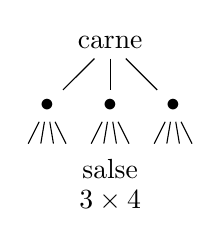
\begin{tikzpicture}[yscale=0.8, xscale=0.8, baseline=(C.base)]
				\node (C) at (0,1) {carne};
				\node (D1) at (-1,0) {$\bullet$};
				\node (D2) at (0,0) {$\bullet$};
				\node (D3) at (1,0) {$\bullet$};
				\draw (C) -- (D1);
				\draw (C) -- (D2);
				\draw (C) -- (D3);
				\node (S) at (0,-1) {salse};
				\draw (D1) -- (-1.3,-0.6);
				\draw (D1) -- (-1.1,-0.6);
				\draw (D1) -- (-0.9,-0.6);
				\draw (D1) -- (-0.7,-0.6);
				\draw (D2) -- (-0.3,-0.6);
				\draw (D2) -- (-0.1,-0.6);
				\draw (D2) -- (0.1,-0.6);
				\draw (D2) -- (0.3,-0.6);
				\draw (D3) -- (0.7,-0.6);
				\draw (D3) -- (0.9,-0.6);
				\draw (D3) -- (1.1,-0.6);
				\draw (D3) -- (1.3,-0.6);
				\node at (0,-1.5) {$3 \times 4$};
			\end{tikzpicture}
			&
			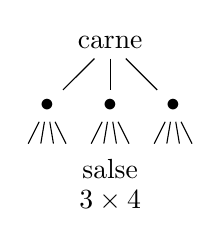
\begin{tikzpicture}[yscale=0.8, xscale=0.8, baseline=(C.base)]
				\node (C) at (0,1) {carne};
				\node (D1) at (-1,0) {$\bullet$};
				\node (D2) at (0,0) {$\bullet$};
				\node (D3) at (1,0) {$\bullet$};
				\draw (C) -- (D1);
				\draw (C) -- (D2);
				\draw (C) -- (D3);
				\node (S) at (0,-1) {salse};
				\draw (D1) -- (-1.3,-0.6);
				\draw (D1) -- (-1.1,-0.6);
				\draw (D1) -- (-0.9,-0.6);
				\draw (D1) -- (-0.7,-0.6);
				\draw (D2) -- (-0.3,-0.6);
				\draw (D2) -- (-0.1,-0.6);
				\draw (D2) -- (0.1,-0.6);
				\draw (D2) -- (0.3,-0.6);
				\draw (D3) -- (0.7,-0.6);
				\draw (D3) -- (0.9,-0.6);
				\draw (D3) -- (1.1,-0.6);
				\draw (D3) -- (1.3,-0.6);
				\node at (0,-1.5) {$3 \times 4$};
			\end{tikzpicture}
			&
			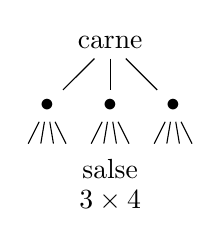
\begin{tikzpicture}[yscale=0.8, xscale=0.8, baseline=(C.base)]
				\node (C) at (0,1) {carne};
				\node (D1) at (-1,0) {$\bullet$};
				\node (D2) at (0,0) {$\bullet$};
				\node (D3) at (1,0) {$\bullet$};
				\draw (C) -- (D1);
				\draw (C) -- (D2);
				\draw (C) -- (D3);
				\node (S) at (0,-1) {salse};
				\draw (D1) -- (-1.3,-0.6);
				\draw (D1) -- (-1.1,-0.6);
				\draw (D1) -- (-0.9,-0.6);
				\draw (D1) -- (-0.7,-0.6);
				\draw (D2) -- (-0.3,-0.6);
				\draw (D2) -- (-0.1,-0.6);
				\draw (D2) -- (0.1,-0.6);
				\draw (D2) -- (0.3,-0.6);
				\draw (D3) -- (0.7,-0.6);
				\draw (D3) -- (0.9,-0.6);
				\draw (D3) -- (1.1,-0.6);
				\draw (D3) -- (1.3,-0.6);
				\node at (0,-1.5) {$3 \times 4$};
			\end{tikzpicture}
		\end{tabular}
	\end{center}
	
	\[
	\#\text{Soluzione} = \#\text{Tipo 1} + \#\text{Tipo 2} + \#\text{Tipo 3}
	\]
	$\hookrightarrow$ stesso risultato dell'altro procedimento
	
	Rendiamo i concetti più chiari con un esempio.\\
	Supponiamo di voler ottenere il \textit{numero di targhe con una sola P}.
	
	In questo caso possiamo suddividere l'insieme ambiente delle targhe con una sola P in quattro sottoinsiemi (tipi):
	\begin{itemize}
		
		\item \textbf{Tipo 1}: targhe con P in prima posizione ($\text{P} - \dots -$).
		
		\item \textbf{Tipo 2}: targhe con P in seconda posizione ($-\text{P} - \dots$).
		
		\item \textbf{Tipo 3}: targhe con P in terza posizione ($-\dots\text{P}-$).
		
		\item \textbf{Tipo 4}: targhe con P in quarta posizione ($-\dots-\text{P}$).
		
	\end{itemize}
	
	Siccome ci rendiamo conto che queste quattro tipologie ricostruiscono l'insieme ambiente (requisito fondamentale per il principio di addizione), la soluzione finale sarà anche qui la somma delle cardinalità dei vari tipi:
	\[
		\#\text{Tipo 1} = \#\text{Tipo 2} = \#\text{Tipo 3} = \#\text{Tipo 4} = 25^3 \times 10^3
	\]
	poiché in tutte le tipologie fissiamo ed escludiamo una e una sola lettera. Di conseguenza:
	\[
		\#\text{Sol} = \#\text{Tipo 1} + \#\text{Tipo 2} + \#\text{Tipo 3} + \#\text{Tipo 4} = 4 \times 25^3 \times 10^3
	\]
	
	E se invece volessimo contare quante sono le targhe con \textit{almeno} una P?
	
	Potremo dividerlo nelle seguenti tipologie:
	\begin{itemize}
		
		\item P in prima e forse altrove;
		
		\item P in seconda e forse altrove;
		
		\item P in terza e forse altrove;
		
		\item P in quarta e forse altrove.
	
	\end{itemize}
	
	Ci rendiamo conto però di un problema: alcune targhe appartengono a più tipologie contemporaneamente. Quando scegliamo male le tipologie possono verificarsi due situazioni:
	\begin{itemize}
		
		\item $\#\text{Sol} < \#T_1 + \#T_2 + \#T_3 + \#T_4$. In questo caso i tipi si dicono \textbf{non esclusivi}, perché possono essere presenti duplicati (intersezioni).
		
		\item $\#\text{Sol} > \#T_1 + \#T_2 + \#T_3 + \#T_4$. In questo caso i tipi si dicono \textbf{non esaustivi}, perché potremmo non aver considerato tutte le effettive combinazioni.
		
	\end{itemize}
	
	Formalizziamo quanto abbiamo visto grazie agli esempi.
	
	Sia $A$ un insieme finito e siano $T_1 \subseteq A, \, T_2 \subseteq A, \, \dots, \, T_k \subseteq A$ dei suoi sottoinsiemi.
	
	\begin{description}
		
		\item [Esaustività:] ogni elemento di $A$ è presente in almeno uno dei $T_i$. Formalmente:
		\[
		A \subseteq T_1 \cup T_2 \cup \dots \cup T_K \implies (\#A \leq \#T_1 + \dots + \#T_K)
		\]
		
		\item [Esclusività:] nessun elemento di $A$ è in più di un $T_i$, ovvero $T_i \cap T_j = \emptyset$ (i $T_i$ e $T_j$ sono disgiunti). Formalmente:
		\[
		T_i \cap T_j = \emptyset \implies (\#A \geq \#T_1 + \dots + \#T_K)
		\]
		
	\end{description}
	
	Vediamo un'applicazione pratica del principio additivo attraverso un problema di conteggio.
	
	Siano $8$ gli atleti in gara, di cui $2$ italiani (IT), $3$ francesi (FR) e $3$ spagnoli (SP). Vogliamo contare tutti gli ordini di arrivo in cui i primi tre atleti hanno nazionalità diverse.
	
	Se vogliamo risolvere il problema utilizzando il principio di addizione, dobbiamo partizionare l'insieme delle soluzioni. Una possibile e corretta partizione si ottiene considerando le diverse sequenze di nazionalità per il podio:
	\[
		\text{IFS} = \{\text{soluzioni con IT in } 1^{\text{a}}, \text{FR in } 2^{\text{a}} \text{ e SP in } 3^{\text{a}}\}
	\]
	e un discorso analogo vale per le altre partizioni possibili (ISF, FIS, SIF, FSI, SFI). In formule, $(a_1, \dots, a_8) \in \text{IFS} \iff a_1 = \text{IT}, a_2 = \text{FR}, a_3 = \text{SP}$.
	
	Calcoliamo in quanti modi possiamo disporre i primi tre atleti scegliendo nazionalità diverse:
	\[
		\text{IFS} = 2 \times 3 \times 3
	\]
	dove:
	\begin{itemize}
		
		\item $2$ corrisponde alle scelte possibili per il primo posto tra i $2$ atleti IT;
		
		\item il primo $3$ corrisponde alle scelte per il secondo posto tra i $3$ atleti FR;
		
		\item il secondo $3$ corrisponde alle scelte per il terzo posto tra i $3$ atleti SP.
		
	\end{itemize}
	
	Questo ragionamento vale per tutte e $6$ le partizioni, in quanto la struttura delle scelte numeriche rimane la stessa. 
	
	Così facendo, tuttavia, stiamo contando solo le prime tre posizioni. Per le restanti $5$ posizioni basterà disporre i $5$ atleti rimanenti nelle $5$ posizioni libere, il che può essere fatto in $5!$ modi.
	
	Il risultato finale sarà dunque dato da:
	\[
		(2 \times 3 \times 3 \times 5!) \times 6
	\]
	dove il primo blocco rappresenta il totale delle disposizioni di una sola partizione, mentre il fattore $6$ indica il numero totale delle partizioni considerate.
	
	\section{Principio di inclusione-esclusione}
	
	Abbiamo usato il principio di addizione per contare gli oggetti di una collezione divisa per tipi, affinché i tipi fossero distinti e mutualmente esclusivi. Possiamo però formulare il principio anche per contare collezioni definite da proprietà disgiuntive ($A$ o $B$) anche nel caso in cui queste non siano mutualmente esclusive.
	
	Consideriamo un insieme $X$ di persone delle quali determiniamo l'identità di genere. Partizioniamo questo insieme in:
	\begin{itemize}
		
		\item $G_1$: maschi e non femmine;
		
		\item $G_2$: femmine e non maschi;
		
		\item $G_3$: femmine e maschi.
	
	\end{itemize}
	Questa è chiaramente una partizione degli individui che si identificano come maschi o come femmine.
	
	In termini insiemistici questa è l'unione $M \cup F$ dell'insieme $M$ dei maschi e dell'insieme $F$ delle femmine. Per il principio di addizione abbiamo che:
	\[
		\#(M \cup F) = \#G_1 + \#G_2 + \#G_3
	\]
	
	E se avessimo invece scritto l'unione come $\#M + \#F$?
	\begin{itemize}
		
		\item Possiamo partizionare $M$ in $M \cap (X \setminus F)$ e $M \cap F$ (che corrisponde a $G_1$);
		
		\item Similmente per $F$ in $F \cap (X \setminus M)$ e $M \cap F$ (che corrisponde a $G_2$);
		
		\item $M \cap F$ corrisponde a $G_3$.
		
	\end{itemize}
	
	Riscrivendo $\#(M \cup F)$ supponendo però che potrebbe essere l'equivalente a scrivere $\#M + \#F$, esce:
	\[
		\#M + \#F = \underbrace{\#\left(M \cap (X \setminus F)\right)}_{\#G_1} + \underbrace{\#\left(M \cap F\right)}_{\#G_3} + \underbrace{\#\left(F \cap (X \setminus M)\right)}_{\#G_2} + \underbrace{\#\left(M \cap F\right)}_{\#G_3}
	\]
	
	Notiamo che stiamo contando due volte $\#(M \cap F)$, dunque per ottenere un'uguaglianza valida a mettere in relazione $M \cup F$ e $M + F$ dovremo semplicemente togliere un conteggio dell'intersezione:
	\[
		\#(M \cup F) = \#M + \#F - \#(M \cap F)
	\]
	
	Questo viene detto \textbf{principio di inclusione-esclusione}, e in questo caso è detto a 2 termini:
	\[
		\#(A \cup B) = \#A + \#B - \#(A \cap B)
	\]
	
	Possiamo però anche vedere il principio di inclusione-esclusione a più termini.
	Consideriamo una classe sottoposta a 3 esami: $C, I, L$. I risultati sono:
	\begin{itemize}
		
		\item $12$ superano $I$;
		
		\item $5$ superano $L$;
		
		\item $8$ superano $C$;
		
		\item $2$ sia $I$ che $L$;
		
		\item $6$ sia $I$ che $C$;
		
		\item $3$ sia $L$ che $C$;
		
		\item $1$ tutti e $3$.
		
	\end{itemize}
	
	Quanti hanno superato almeno un test?
	Posto $I = \{\text{studenti che superano } I\}$, $L = \{\text{studenti che superano } L\}$, $C = \{\text{studenti che superano } C\}$.
	
	Come abbiamo imparato, non possiamo dire che 
	\[
		\#\text{SOL} = \#I + \#L + \#C
	\]
	perché staremmo contando tanti casi duplicati. Togliamo dunque le intersezioni tra gli insiemi:
	\[
		\#I + \#L + \#C - \#(I \cap L) - \#(I \cap C) - \#(L \cap C)
	\]
	
	Siamo vicini alla soluzione, in quanto in questo calcolo abbiamo contato una volta gli studenti che superano tutti e $3$ i test, ma poi li abbiamo tolti con le varie intersezioni. Aggiungiamo dunque la tripla intersezione:
	\[
		\#\text{SOL} = \#I + \#L + \#C - \#(I \cap L) - \#(I \cap C) - \#(L \cap C) + \#(I \cap L \cap C)
	\]
	
	Generalizzando...
	\[
		\text{PIE}_3 = \#A + \#B + \#C - \#(A \cap B) - \#(A \cap C) - \#(B \cap C) + \#(A \cap B \cap C)
	\]
	
	Possiamo generalizzare ancora di più formulando un $\text{PIE}_n$ con le seguenti osservazioni:
	\begin{enumerate}
		
		\item Includo (sommo) le cardinalità dei singoli;
		
		\item Escludo (sottraggo) le cardinalità delle intersezioni a due a due;
		
		\item Includo (sommo) le cardinalità delle intersezioni a tre a tre;
		
		\item Escludo (sottraggo) le cardinalità delle intersezioni a quattro termini;
		
		\item $\dots$
		
	\end{enumerate}
	
	Possiamo dunque formulare una formula generale per $n$ insiemi.
	Siano $A_1, \dots, A_n$ insiemi finiti. La loro unione contiene esattamente:
	\[
		\sum_{i=1}^{n} \#A_i - \sum_{1 \le i_1 < i_2 \le n} \#(A_{i_1} \cap A_{i_2}) + \sum_{1 \le i_1 < i_2 < i_3} \#(A_{i_1} \cap A_{i_2} \cap A_{i_3}) - \dots + (-1)^{n-1} \#(A_1 \cap \dots \cap A_n)
	\]
	con la regola per cui se $n$ è pari allora il segno è $+$, mentre se $n$ è dispari il segno è $-$.
	
	\section{Combinazioni semplici}
	
	Per introdurre lo studio delle combinazioni semplici, possiamo partire da una regola intuitiva, nota come la \emph{regola del pastore}: per contare le pecore in un gregge, conta le zampe e dividi per $4$. 
	
	Sembra una regola banale, ma se proviamo a generalizzarla otteniamo una nuova e importante figura della calcolatoria. Consideriamo ad esempio una gara con $8$ atleti, in cui ci interessano solo le qualificazioni dei primi $3$ che potranno poi proseguire nella fase successiva.
	
	In questo caso non ci interessa l'ordine di arrivo, bensì solo quali atleti si sono qualificati. Adesso dunque non contiamo più le sequenze ordinate, bensì i sottoinsiemi dell'insieme di partenza. 
	Ricordiamo infatti che:
	\[
		(a, b, c) \neq (c, b, a) \quad (\text{parentesi tonde: l'ordine conta})
	\]
	mentre
	\[
		\{a, b, c\} = \{b, c, a\} \quad (\text{parentesi graffe: l'ordine non conta})
	\]
	
	Per risolvere il problema, contiamo il numero di sequenze ordinate senza ripetizioni $D_{8,3}$ e dividiamo per il numero di permutazioni possibili ($3!$), dato che le combinazioni duplicate vengono così conteggiate una sola volta. Otteniamo quindi:
	\[
		\text{\# qualifiche} = \frac{D_{8,3}}{3!}
	\]
	
	\begin{definizione}{Insieme dei $n$-sottoinsiemi}{}
		
		Sia $A$ un insieme e sia $n \ge 0$ un numero naturale. Un $n$-sottoinsieme di $A$ è un sottoinsieme di $A$ con esattamente $n$ elementi. Indichiamo con $[A]^n$ l'insieme di tutti i $n$-sottoinsiemi di $A$.
		
	\end{definizione}
	
	Generalizzando quanto visto, definiamo le \textbf{combinazioni semplici} di ordine $k$ su $n$ come i sottoinsiemi di $k$ elementi scelti da un insieme di $n$ elementi. La formula generale è data da:
	\[
		C_{n,k} = [A]^k = \binom{n}{k} = \frac{D_{n,k}}{k!} = \frac{n!}{(n-k)! \cdot k!}
	\]
	dove $A$ è un insieme con $n$ elementi.
	
	Per comprendere l'applicazione pratica di questo principio, consideriamo un problema concreto.
	Supponiamo di avere $80$ rappresentanti di religioni differenti: $50$ cristiani, $20$ induisti e $10$ buddisti. Vogliamo determinare quante delegazioni di $5$ persone si possono formare in modo che vi sia almeno un rappresentante per ogni confessione.
	
	Un approccio diretto sarebbe troppo laborioso, perciò procediamo con il \textbf{passaggio al complemento}. Il numero totale di delegazioni possibili è dato dal coefficiente binomiale $\binom{80}{5}$. Le delegazioni ``cattive'', ovvero quelle in cui manca almeno un rappresentante di una confessione (quindi nessun cristiano, oppure nessun induista, oppure nessun buddista), possono essere viste come l'unione di tre insiemi:
	\[
	A = \{5 \text{ senza CR}\}, \quad B = \{5 \text{ senza IND}\}, \quad C = \{5 \text{ senza BUD}\}
	\]
	Applicando il principio di inclusione-esclusione per tre insiemi ($\operatorname{PIE}_3$), vogliamo calcolare la cardinalità dell'unione:
	\[
	\#(A \cup B \cup C) = \#A + \#B + \#C - \#(A \cap B) - \#(A \cap C) - \#(B \cap C) + \#(A \cap B \cap C)
	\]
	dove in questo caso specifico $\#(A \cap B \cap C) = \emptyset$, perché non ha senso una delegazione senza alcun rappresentante.
	Sostituendo i valori otteniamo:
	\[
	\binom{80-50}{5} + \binom{80-20}{5} + \binom{80-10}{5} - \binom{50}{5} - \binom{20}{5} - \binom{10}{5}
	\]
	Sottrarremo poi questo valore dal totale $\binom{80}{5}$ per trovare le delegazioni desiderate.
	
	\subsection{Proprietà dei coefficienti binomiali}
	
	Analizziamo alcune proprietà notevoli e identità combinatorie relative ai coefficienti binomiali attraverso un esempio pratico.
	
	Supponiamo di avere $80$ studenti e di voler formare una delegazione di $4$ rappresentanti, di cui uno con il ruolo di portavoce. Possiamo procedere in due modi equivalenti:
	
	\begin{enumerate}
		
		\item \textbf{Primo modo}: Scelgo prima i $4$ rappresentanti tra gli $80$ studenti, e successivamente scelgo il portavoce tra i $4$ prescelti. Questo corrisponde al calcolo $\binom{80}{4} \times 4$.
		
		\item \textbf{Secondo modo}: Scelgo prima il portavoce tra gli $80$ studenti, e poi scelgo i restanti $3$ membri della delegazione tra i $79$ studenti rimasti. Questo corrisponde al calcolo $80 \times \binom{79}{3}$.
		
	\end{enumerate}
	
	A livello numerico otteniamo l'uguaglianza:
	\[
		\binom{80}{4} \times 4 = 80 \times \binom{79}{3}
	\]
	la quale può essere riscritta in termini di coefficienti binomiali come $\binom{80}{4} \binom{4}{1} = \binom{80}{1} \binom{79}{3}$.
	
	Se invece i portavoce fossero $2$, i due modi corrisponderebbero rispettivamente a $\binom{80}{4} \times \binom{4}{2}$ e $\binom{80}{2} \times \binom{78}{2}$.
	
	Generalizzando questo ragionamento, otteniamo l'identità generale:
	\[
		\binom{n}{k} \binom{k}{m} = \binom{n}{m} \binom{n-m}{k-m}
	\]
	
	\begin{proposizione}{}{}
		
		I $k$-sottoinsiemi di un insieme di $n$ elementi sono in corrispondenza biunivoca con i loro complementari. Di conseguenza, vale la simmetria dei coefficienti binomiali:
		\[
			\binom{n}{k} = \binom{n}{n-k}
		\]
		
	\end{proposizione}
	
	\begin{dimostrazione}{}{}
		
		Sia $A$ un insieme con $|A| = n$ e sia $S \subseteq A$ un $k$-sottoinsieme, ovvero $S = \{a_1, \dots, a_k\}$. 
		Il complemento di $S$ in $A$, denotato con $A \setminus S$, è l'insieme degli elementi che appartengono ad $A$ ma non a $S$. 
		Poiché stiamo rimuovendo $k$ elementi da un totale di $n$ elementi, la cardinalità del complementare sarà esattamente:
		\[
		|A \setminus S| = n - k
		\]
		Ogni volta che scegliamo un $k$-sottoinsieme $S$, stiamo univocamente determinando un $(n-k)$-sottoinsieme (il suo complemento). 
		Il numero dei $k$-sottoinsiemi di un insieme di $n$ elementi è dunque uguale al numero dei loro complementi, che corrisponde al numero degli $(n-k)$-sottoinsiemi dello stesso insieme.
		Da ciò discende la nota proprietà simmetrica, come ad esempio $\binom{100}{3} = \binom{100}{97}$.
		
	\end{dimostrazione}
	
	\begin{osservazione}{}{}
		
		Ogni $k$-sottoinsieme ha una corrispondenza diretta ($1:1$, iniettività) con un $(n-k)$-sottoinsieme.
		
	\end{osservazione}
	
	Stiamo partizionando l'insieme dei $k$-sottoinsiemi di $A$, che indichiamo con $[A]^k$.
	Contiamo ora i sottoinsiemi utilizzando una partizione in due tipi distinti:
	
	\begin{itemize}
		
		\item \textbf{Tipo 1 (inclusivi)}: insiemi in cui è sempre presente un elemento speciale (che chiamiamo ad esempio $PN$). Due insiemi di questo tipo differiscono solo per le restanti $n-1$ scelte. Rimuovendo temporaneamente l'elemento $PN$, dobbiamo scegliere $k-1$ elementi tra i restanti $n-1$ totali, ottenendo il coefficiente binomiale $\binom{n-1}{k-1}$.
		
		\item \textbf{Tipo 2 (esclusivi)}: insiemi in cui l'elemento $PN$ non è mai presente. Di conseguenza, dobbiamo scegliere $k$ elementi tra i restanti $n-1$ disponibili, ottenendo $\binom{n-1}{k}$.
		
	\end{itemize}
	
	Sommando i contributi dei due tipi, e sapendo che il totale dei sottoinsiemi di $k$ elementi è dato semplicemente da $\binom{n}{k}$, otteniamo la celebre identità:
	\[
		\binom{n}{k} = \binom{n-1}{k-1} + \binom{n-1}{k}
	\]
	
	\subsection{Generalizzazione}
	Sia $A = \{a_1, a_2, \dots, a_n\}$. Partizioniamo $[A]^k$ fissando due elementi distinti $a, b \in A$ e analizzando tutte le possibili combinazioni della loro presenza all'interno dei sottoinsiemi $S$:
	
	\begin{enumerate}
		\item $T_1 = \{a \in S, b \in S\}$, da cui otteniamo $\binom{n-2}{k-2}$
		\item $T_2 = \{a \in S, b \notin S\}$, da cui otteniamo $\binom{n-2}{k-1}$
		\item $T_3 = \{a \notin S, b \in S\}$, da cui otteniamo $\binom{n-2}{k-1}$
		\item $T_4 = \{a \notin S, b \notin S\}$, da cui otteniamo $\binom{n-2}{k}$
	\end{enumerate}
	
	\section{Buona traduzione}
	Supponiamo che due mercanti vogliano comunicare segretamente le città in cui vendere i propri prodotti, senza essere intercettati da terzi.
	
	Tra i modi possibili, ne segnaliamo uno in particolare:
	\begin{itemize}
		\item Si mettono d'accordo sulla sequenza ordinata delle città da visitare: $(c_1, c_2, \dots, c_n)$.
		\item In seguito possono usare una sequenza (stringa) binaria in cui ogni cifra verrà messa in corrispondenza di una città, in modo che:
		\begin{itemize}
			\item $1$: città presente;
			\item $0$: città assente.
		\end{itemize}
	\end{itemize}
	
	Possiamo applicare questo concetto, insieme alle combinazioni, per determinare il numero di sottoinsiemi di un insieme di $n$ elementi.
	\[
	\mathcal{P}(A) = \{S \mid S \subseteq A\}
	\]
	dove $\mathcal{P}(A)$ è l'insieme potenza, ossia l'insieme di tutti i sottoinsiemi. La sua cardinalità è data da:
	\[
	\#\mathcal{P}(A) = 2^n = \sum_{i=0}^{n} \binom{n}{i}
	\]
	
	La "buona traduzione" si basa su tre concetti fondamentali, dati una funzione $T: X \to Y$:
	\begin{itemize}
		\item Ogni elemento $x \in X$ viene tradotto in esattamente un elemento $y \in Y$.
		\item Ogni elemento $y \in Y$ si ottiene come traduzione di almeno un elemento $x \in X$.
		\item Elementi distinti di $X$ hanno traduzioni diverse:
		\[
		\forall x, x' \in X, \quad x \neq x' \implies T(x) \neq T(x')
		\]
	\end{itemize}
	
	\section{Combinazioni con ripetizioni}
	
	Supponiamo che il pastore Ettore debba distribuire $3$ pasticche del pastore a $2$ ragazzi.
	Le clausole sono le seguenti:
	\begin{itemize}
		\item Le pasticche sono identiche;
		\item Non per forza ogni ragazzo deve ricevere qualcosa.
	\end{itemize}
	
	Proviamo a rappresentare graficamente la soluzione in due modi:
	
	\begin{center}
		\begin{tabular}{c|c}
			\textbf{Giorgio} & \textbf{Marco} \\
			\hline
			0 & 3 \\
			1 & 2 \\
			2 & 1 \\
			3 & 0
		\end{tabular}
		\hspace{2cm}
		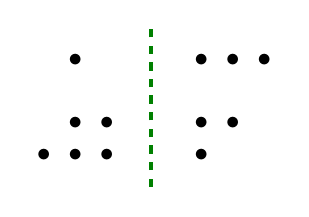
\begin{tikzpicture}[scale=0.8, baseline={(0, 0.50cm)}]
			\node at (0,1.5) {$\bullet$};
			\node at (0,0.5) {$\bullet$}; \node at (0.5,0.5) {$\bullet$};
			\node at (-0.5,0) {$\bullet$}; \node at (0,0) {$\bullet$}; \node at (0.5,0) {$\bullet$};
			
			\draw[very thick, green!50!black, dashed] (1.2,-0.5) -- (1.2,2);
			
			\node at (2,1.5) {$\bullet$}; \node at (2.5,1.5) {$\bullet$}; \node at (3,1.5) {$\bullet$};
			\node at (2,0.5) {$\bullet$}; \node at (2.5,0.5) {$\bullet$};
			\node at (2,0) {$\bullet$};
		\end{tikzpicture}
	\end{center}
	
	Questa rappresentazione indica le sequenze ordinate di $3$ pallini e $1$ stanghetta.
	
	E se invece il pubblico fosse di $6$ persone e dovessero essere consegnate $7$ pasticche?
	Si potrebbero comunque rappresentare come sequenze di $7$ palline e $(6-1) = 5$ stanghette, per un totale di $7 + 5 = 12$ elementi.
	
	Supponiamo di avere una rappresentazione del genere:
	\[
	\underbrace{\bullet \, \bullet}_{2} \, | \, \underbrace{\bullet}_{1} \, | \, \underbrace{\bullet}_{1} \, | \, \underbrace{\bullet \, \bullet \, \bullet}_{3} \, | \, | \, \underbrace{\quad}_{0} \, | \, \underbrace{\quad}_{0}
	\]
	
	Osserviamo che per determinare le varie sequenze ci basterebbe anche sapere \textit{solo} la posizione dei pallini.
	In questo caso l'ordine non conta in quanto è stato fissato a priori, scegliendo $7$ indici tra i $12$ elementi totali: i $7$-sottoinsiemi di un insieme di $12$ elementi.
	
	Ad esempio, per l'es. 1: $\{1, 2, 4, 6, 8, 9, 10\}$.
	La soluzione sarà dunque $\binom{12}{7} = \binom{12}{5}$ come sappiamo per le relazioni tra $\mathcal{C}_{n,k}$.
	
	In generale, con il metodo \textbf{Stars \& Bars}, possiamo definire le formule:
	\[
	\binom{p+r-1}{p} = \binom{n+k-1}{k}
	\qquad
	\binom{p+r-1}{p-1} = \binom{n+k-1}{k-1}
	\]
	dove $p$ (o $n$) rappresenta le pasticche e $r$ (o $k$) rappresenta le persone.
	
	Vediamo un altro esempio di calcolo combinatorio applicato alle equazioni in interi.
	
	\begin{itemize}
		\item Quante sono le soluzioni intere positive della seguente equazione:
		\[
		x_1 + x_2 + x_3 + x_4 + x_5 = 10
		\]
		
		Applichiamo il principio visto in precedenza, dove $10$ rappresentano le unità e le $5$ incognite i ragazzi:
		\[
		\binom{10 + 5 - 1}{5 - 1} = \binom{10 + 5 - 1}{10}
		\]
		
		\item E se invece chiedessimo le soluzioni dove $x_i > 0$?
		Beh, in questo caso ogni $x_i \geq 1$. Suddividiamo il procedimento in passaggi:
		\begin{enumerate}
			\item Diamo una unità \textbf{subito} ad ogni variabile.
			\item Contiamo i modi di distribuire le restanti $5$ ($= 10 - 5$) unità alle $5$ variabili:
			\[
			\binom{5 + 5 - 1}{5 - 1} = \binom{9}{4}
			\]
		\end{enumerate}
		Nel primo passaggio abbiamo rimosso il vincolo, poi abbiamo proceduto come da manuale.
	\end{itemize}
	
	Altro esempio:
	\begin{itemize}
		\item Soluzioni dell'equazione $x + y + z = 11$, tali che $x, y, z \leq 4$.
		
		\begin{enumerate}
			\item \textbf{Passaggio al complemento}
			
			Costruisco la partizione tale che:
			\[
			A = \{ \text{dove } x > 4 \}, \quad B = \{ \text{dove } y > 4 \}, \quad C = \{ \text{dove } z > 4 \}
			\]
			Per l'insieme $A$: diamo subito $5$ unità ad $x$ così soddisfo il vincolo, ottenendo $\binom{11 - 5 + 3 - 1}{3 - 1}$.
			Per $B$ e $C$ vale lo stesso discorso, quindi $\#A = \#B = \#C$.
			
			Per costruire la partizione usiamo il principio di inclusione-esclusione ($PIE_3$):
			\[
			\#A + \#B + \#C - \#(A \cap B) - \#(A \cap C) - \#(B \cap C) + \#(A \cap B \cap C)
			\]
			\begin{itemize}
				\item $\emptyset$, in quanto non possono avere tutti e tre unità $> 4$ avendo come massimo $11$.
				\item Quando $y > 4$ e $z > 4$, abbiamo sequenze del tipo $(1, 5, 5), (0, 5, 6), (0, 6, 5)$.
			\end{itemize}
			
			\item \textbf{Sottraiamo il complemento alle soluzioni totali.}
		\end{enumerate}
	\end{itemize}
	
	\chapter{Funzioni}
	
	In informatica parliamo di funzioni quando, ad un input di qualsiasi tipo (numerico, simbolico, \dots) associamo un solo output.
	
	In maniera più astratta possiamo invece dire che una funzione è un'associazione tra elementi di $A$ ed elementi di $B$ tali che ad ogni elemento $a \in A$ viene associato uno e un solo elemento $b \in B$, che indichiamo con $f(a)$ (chiamato anche \textbf{immagine di $a$ sotto la funzione $f$} o \textbf{valore di $f$ sull'argomento $a$}).
	
	Facciamo un esempio:
	\begin{itemize}
		\item Vogliamo contare in quanti modi posso distribuire $8$ giochi distinti a $5$ bambini. Siccome i giochi sono diversi non posso risolverlo con le disposizioni con ripetizione. Possiamo schematizzare in insiemi nel seguente modo:
		\[
		\text{giochi} = \{g^1, g^2, g^3, \dots, g^8\}, \quad \text{bimbi} = \{b_1, b_2, \dots, b_5\}
		\]
		Dove "giochi" sarà il dominio (dato che posso assegnare il singolo gioco ad un solo bambino) mentre "bimbi" sarà il codominio, in quanto un bambino può ricevere più di un gioco (o anche nessuno).
		Le possibilità saranno dunque $(\#\text{bimbi})^{\#\text{giochi}}$.
	\end{itemize}
	
	Andiamo ad ampliare la definizione fornita precedentemente in modo più matematico e rigoroso:
	\[
	f: A \to B
	\]
	è un insieme di coppie ordinate $(a, b)$ con $a \in A$ e $b \in B$ tale che per ogni $a \in A$ esiste un unico $b \in B$ tale che $(a, b) \in f$.
	
	Per esempio, $f: \Z \to \Z$, $f(x) = x - 1$ è una funzione ben definita, in quanto per ogni elemento del dominio è associato uno e un solo elemento del codominio.
	
	Al contrario, per $g: \N \to \N$, $g(n) = n - 1$ non è ben definita in quanto $x = 0$ non ha una corrispondenza nel codominio.
	Possiamo aggiustarla scrivendo $g: \N \setminus \{0\} \to \N$ oppure $g: \N \to \N \cup \{-1\}$.
	
	\section{Iniettività, suriettività e biettività}
	
	Riprendiamo i concetti fondamentali relativi alle funzioni per analizzarli con maggiore formalismo.
	
	\begin{definizione}{Iniettività}{}
		Una funzione $f: A \to B$ si dice \textbf{iniettiva} se non esistono $a, a' \in A$ con $a \neq a'$ tali che $f(a) = f(a')$.
		Equivalentemente, possiamo dire che ad ogni immagine corrisponde una e una sola pre-immagine, ovvero:
		\[
		\forall a, a' \in A, \, a \neq a' \implies f(a) \neq f(a')
		\]
		In modo analogo, la condizione può essere scritta come: se $f(a) = f(a')$, allora $a = a'$.
	\end{definizione}
	
	\begin{definizione}{Suriettività}{}
		Una funzione $f: A \to B$ si dice \textbf{suriettiva} se ogni elemento del codominio $B$ è immagine di almeno un elemento del dominio $A$. Formalmente:
		\[
		B \subseteq \operatorname{Im}(f) \quad \text{oppure} \quad \forall b \in B, \, \exists a \in A \text{ t.c. } f(a) = b
		\]
	\end{definizione}
	
	\begin{definizione}{Biettività}{}
		Una funzione che sia contemporaneamente suriettiva e iniettiva si dice \textbf{biettiva} (o biunivoca).
	\end{definizione}
	
	\section{Funzioni inverse e pre-immagini}
	
	Preso un elemento $b \in B$, vogliamo trovare l'insieme degli elementi del dominio tali che la loro immagine sia $b$, ovvero l'insieme $\{a \in A \mid f(a) = b\}$.
	Tale insieme viene indicato come controimmagine o pre-immagine. 
	
	Sia $f: A \to B$ e sia $y \subseteq B$, definiamo la pre-immagine come:
	\[
	f^{-1}(y) = \{a \in A \mid f(a) = y\}
	\]
	Notiamo che $f^{-1}(b)$ può anche essere un insieme vuoto se $b$ non appartiene all'immagine della funzione.
	
	Consideriamo ora due elementi distinti del codominio $b_I, b_{II} \in B$ con $b_I \neq b_{II}$. Le loro pre-immagini $f^{-1}(b_I)$ e $f^{-1}(b_{II})$ sono disgiunte. Se infatti per assurdo la loro intersezione non fosse vuota, esisterebbe un elemento $a \in A$ tale che $a \in f^{-1}(b_I)$ e $a \in f^{-1}(b_{II})$, il che significherebbe $f(a) = b_I$ e $f(a) = b_{II}$, contro l'ipotesi che $b_I \neq b_{II}$.
	Possiamo quindi concludere che, al variare di $b \in B$, le pre-immagini $f^{-1}(b)$ sono a due a due disgiunte.
	
	Definiamo l'insieme famiglia delle pre-immagini come:
	\[
	\mathcal{F} = \{f^{-1}(b) \mid b \in B\}
	G\]
	Per ogni $b \in B$ si ha $f^{-1}(b) \subseteq A$ e per ogni $b \neq b'$ si ha $f^{-1}(b) \cap f^{-1}(b') = \emptyset$. Inoltre, per ogni elemento $a \in A$ esiste un $b \in B$ tale che $f(a) = b$, ovvero $a \in f^{-1}(b)$.
	
	Possiamo riassumere dicendo che, data una funzione $f: A \to B$, la famiglia $\mathcal{F}$ costituisce una \textbf{partizione} dell'insieme $A$.
	
	\section{Funzioni e operatori insiemistici}
	
	Possiamo formulare proprietà generali riguardanti il comportamento delle funzioni come oggetti insiemistici.
	
	Se $f: X \to Y$ e $A, B \subseteq X$, sono sempre ben definiti i seguenti insiemi: $f(A), f(B), A \cap B, f(A \cap B), f(A) \cap f(B)$.
	
	Possiamo chiederci quali relazioni incorrano tra l'intersezione delle immagini ($f(A) \cap f(B)$) e l'immagine dell'intersezione tra i due insiemi ($f(A \cap B)$).
	
	\begin{osservazione}{}{}
		Vale la seguente inclusione:
		\[
		f(A \cap B) \subseteq f(A) \cap f(B)
		\]
	\end{osservazione}
	
	\begin{dimostrazione}{Dimostrazione}{}
		Sia $z \in f(A \cap B)$. Per definizione di immagine, sappiamo che esiste $w \in (A \cap B)$ tale che $f(w) = z$. Allora esiste $w \in A$ tale che $f(w) = z$ e un $w' \in B$ tale che $f(w') = z$ (basta scegliere lo stesso elemento, siccome per l'intersezione $w$ appartiene sia ad $A$ che a $B$).\\
		Dunque $z \in f(A)$ e $z \in f(B)$, da cui $z \in f(A) \cap f(B)$.
	\end{dimostrazione}
	
	Tuttavia non vale in generale il viceversa. Supponiamo $x \neq x' \in X$ tali che $f(x) = f(x')$. Ponendo $A = \{x\}$ e $B = \{x'\}$, abbiamo che $f(x) \in f(A) \cap f(B)$ ma $f(A \cap B) = \emptyset$, quindi non possono equivalersi.
	
	Per quanto riguarda il contrario, ci chiediamo se valga la relazione opposta:
	\[
	f(A) \cap f(B) \subseteq f(A \cap B) \quad \text{valida solo se } f \text{ è iniettiva}
	\]
	
	Questo avviene generalmente perché un $y \in Y$ è associato a due valori $x_1, x_2 \in X$. Se invece $f$ fosse iniettiva, allora per un valore di $y$ abbiamo una sola $x$ e dunque l'uguaglianza è valida.
	
	\begin{dimostrazione}{}{}
		\textbf{Tesi}: $f(A \cup B) = f(A) \cup f(B)$
		
		\smallbreak
		Sia $y \in f(A \cup B)$, allora esiste $x \in (A \cup B)$ tale che $f(x) = y$. Per definizione di unione, $x \in A \lor x \in B$. Se $x \in A$, $y \in f(A)$; se $x \in B$, $y \in f(B)$. L'inclusione è vera.
		
		\smallbreak
		\textbf{Tesi}: $f(A) \cup f(B) = f(A \cup B)$
		
		\smallbreak
		Sia $y \in f(A) \cup f(B)$. Allora $y \in f(A) \lor y \in f(B)$. Nel primo caso esiste $x \in A$ con $f(x) = y$; dato che $A \subseteq A \cup B$, quel $x \in A \cup B$, quindi $y \in f(A \cup B)$. Anche in questo caso l'inclusione è vera.
	\end{dimostrazione}
	
	Quando parliamo di operazioni insiemistiche, intendiamo le operazioni che si possono svolgere tra le coppie $(x, f(x))$ di due o più funzioni.
	
	Siano $f, g \subseteq X \times Y$:
	\begin{itemize}
		\item $f \cup g$ è $\{(x, y) \mid (x, y) \in f \lor (x, y) \in g\}$.
	\end{itemize}
	Questa unione rischia di non essere più una funzione in quanto potrebbe accadere che ad uno stesso valore $x$ vengano assegnati $2$ valori distinti $y$. Sostanzialmente, per essere una funzione, gli intervalli di definizione delle due funzioni devono essere disgiunti.
	
	\begin{itemize}
		\item $f \cap g$ è $\{(x, y) \mid (x, y) \in f \land (x, y) \in g\}$.
	\end{itemize}
	Prendiamo solo le coppie comuni ed è dunque impossibile che queste non costituiscano una funzione in quanto $f$ e $g$ lo sono.
	
	\section{Composizione di funzioni}
	
	\begin{definizione}{Funzione composta}{}
		Siano $f: X \to Y$ e $g: Y \to Z$. La funzione composta di $f$ e $g$ è la funzione $h: X \to Z$ definita ponendo $h(x) = g(f(x)),\, \forall x \in X$ e si denota con $g \circ f$ ($g$ composta con $f$).
	\end{definizione}
	
	Si nota semplicemente che la composizione è possibile solo se $f(X) \subseteq Y$, ossia l'immagine di $f$ è contenuta nel dominio di $g$.
	
	\begin{osservazione}{}{}
		Siano $f(x) = 2x + 3$ e $g(y) = y^2$. Si ha che $(g \circ f)(x) = g(f(x)) = (2x+3)^2$, tuttavia $(f \circ g)(x) = f(g(x)) = 2x^2 + 3$, quindi la composizione \textbf{non è commutativa}. Vale però l'associatività: $h \circ (g \circ f) = (h \circ g) \circ f$.
	\end{osservazione}
	
	\begin{proposizione}{}{}
		Se $f$ e $g$ sono iniettive, allora $g \circ f$ è iniettiva.
	\end{proposizione}
	\begin{dimostrazione}{}{}
		Dimostriamo per assurdo. Supponiamo esista $z \in Z$ tale che $\exists x \neq x' \in X$ con $(g \circ f)(x) = (g \circ f)(x')$, che possiamo riscrivere come $g(f(x)) = g(f(x'))$.
		Dato che $g$ è iniettiva, allora $f(x) = f(x')$ per far sì che la composta non sia iniettiva. Ma allora anche $f$, essendo iniettiva, impone che $f(x) = f(x') \iff x = x'$. Ma abbiamo trovato una contraddizione perché avevamo stabilito $x \neq x'$.
	\end{dimostrazione}
	
	\begin{proposizione}{}{}
		Se $f$ e $g$ sono suriettive, allora $g \circ f$ è suriettiva.
	\end{proposizione}
	\begin{dimostrazione}{}{}
		Vogliamo dimostrare che $\forall z \in Z \,\, \exists x \in X$ con $(g \circ f)(x) = z$.
		\begin{itemize}
			\item Poiché $g$ è suriettiva, $\exists y \in Y$ t.c. $g(y) = z$.
			\item Poiché $f$ è suriettiva, $\exists x \in X$ t.c. $f(x) = y$.
		\end{itemize}
		Allora $g(f(x)) = g(y) = z$, dunque la funzione è suriettiva.
	\end{dimostrazione}
	
	Per la biettività basta unire le due dimostrazioni precedenti.
	% --- NEW PAGE ---
	
	\section{Caratterizzazione di iniezione}
	
	\begin{teorema}{Caratterizzazione di iniezione}{}
		Se $f: X \to Y$ è iniettiva, allora esiste $g: Y \to X$ tale che $(g \circ f): X \to X$ è l'identità su $X$ ($\operatorname{id}_X$), ossia $\forall x \in X, \, (g \circ f)(x) = x$.
	\end{teorema}
	
	\begin{dimostrazione}{}{}
		Poiché $f$ è iniettiva, $\forall y \in Y$ esiste al più un $x \in X$ tale che $f(x) = y$.
		Definiamo ora $g: Y \to X$ come:
		\[
		g(y) =
		\begin{cases}
			\text{l'unica } x \text{ associata tale che } f(x) = y, & \text{se } y \in f(X) \\
			\text{qualsiasi elemento } x \in X, & \text{se } y \notin f(X)
		\end{cases}
		\]
		Questa definizione funziona perché $f(X) \subseteq Y$, quindi nella definizione di $g(y)$ teniamo conto solo dei valori $y \in Y$ che hanno corrispondenza con un unico $x \in X$.
	\end{dimostrazione}
	
	E il contrario? Se esiste $g: Y \to X$ tale che $(g \circ f): X \to X$ è $\operatorname{id}_X$, $f$ è iniettiva?
	
	\begin{dimostrazione}{}{}
		Supponiamo che $f$ non sia iniettiva. Allora esistono $x \neq x' \in X$ tali che $f(x) = f(x')$.
		Ma sappiamo che $g(f(x)) = \operatorname{id}_X(x) = x$ e $g(f(x')) = \operatorname{id}_X(x') = x'$. Sapendo ciò, dato che $g$ è una funzione, per uno stesso valore non possiamo avere immagini diverse e dunque $g(f(x)) = g(f(x'))$, cioè $x = x'$, che contraddice la nostra supposizione.
	\end{dimostrazione}
	
	Infine, $f: X \to Y$ è iniettiva se e solo se esiste $g: Y \to X$ tale che $(g \circ f): X \to X = \operatorname{id}_X$.
	
	\begin{osservazione}{}{}
		Consideriamo ad esempio $f: \{1, 2, 3\} \to \{a, b, c, d\}$, con $f(1) = a$, $f(2) = b$, $f(3) = c$.
		Possiamo definire $g: f(\{1, 2, 3\}) \to \{1, 2, 3\}$ tale che:
		\[
		g(a) = 1, \quad g(b) = 2, \quad g(c) = 3
		\]
		Verifichiamo la composizione:
		\[
		(g \circ f)(1) = g(a) = 1, \quad (g \circ f)(2) = g(b) = 2, \quad (g \circ f)(3) = g(c) = 3
		\]
	\end{osservazione}
	
	\section{Caratterizzazione di suriezione}
	
	\begin{teorema}{Caratterizzazione di suriezione}{}
		Sia $f: X \to Y$ una funzione. $f$ è suriettiva se e solo se esiste una funzione $g: Y \to X$ tale che la funzione composta $(f \circ g): Y \to Y$ sia l'identità su $Y$ ($\operatorname{id}_Y$), ossia $\forall y \in Y, \, (f \circ g)(y) = y$.
	\end{teorema}
	
	\begin{dimostrazione}{}{}
		Dimostriamo dapprima che se $f$ è suriettiva, allora esiste tale funzione $g$. Poiché $f$ è suriettiva, $\forall y \in Y, \, \exists x \in X$ tale che $f(x) = y$. Dobbiamo costruirci $g(y)$ in modo che rispetti la proposizione: poniamo $g(y) = \text{uno degli elementi } x \in X \text{ t.c. } f(x) = y$. Questa scelta avviene sempre dato che ogni $y \in Y$ proviene da un $x \in X$ mediante $f$, in quanto la funzione è suriettiva.
		Verifichiamo la composizione:
		\[
		(f \circ g)(y) = f(g(y)) = f(x) = y
		\]
		
		Dimostriamo ora l'implicazione inversa: supponiamo che esista $g: Y \to X$ tale che $(f \circ g): Y \to Y$ sia l'identità. Vogliamo dimostrare che $f$ è suriettiva.
		Supponiamo per assurdo che $f$ non sia suriettiva. Ciò significa che esiste un $y \in Y$ tale che non esiste alcun $x \in X$ per cui $f(x) = y$.
		Se applichiamo la funzione composta a questo elemento $y$:
		\[
		(f \circ g)(y) = f(g(y)) = y
		\]
		ma avevamo detto che $y \notin f(X)$, ottenendo così una contraddizione. La funzione deve quindi essere suriettiva.
	\end{dimostrazione}
	
	Mostriamo un esempio chiarificatore per comprendere la costruzione della funzione inversa destra:
	
	Sia $f: \{1, 2, 3, 4\} \to \{a, b, c\}$ definita da $f(1) = a$, $f(2) = b$, $f(3) = c$ e $f(4) = c$.
	La funzione $f$ è suriettiva in quanto $f(X) = \{a, b, c\} = Y$.
	Possiamo definire una funzione $g: Y \to X$ come $g(a) = 1$, $g(b) = 2$ e $g(c) = 3$.
	Verifichiamo la composizione sugli elementi del codominio:
	\[
	f(g(a)) = a, \quad f(g(b)) = b, \quad f(g(c)) = c
	\]
	% --- NEW PAGE ---
	
	\section{Caratterizzazione di biezione}
	
	\begin{teorema}{Caratterizzazione di biezione}{}
		Sia $f: X \to Y$ biettiva e sia $g: Y \to X$ tale che $(g \circ f): X \to X = \operatorname{id}_X$ e $(f \circ g): Y \to Y = \operatorname{id}_Y$.
	\end{teorema}
	
	\begin{dimostrazione}{}{}
		Supponiamo che $(f \circ g): Y \to Y \neq \operatorname{id}_Y$. Questo significa che per almeno un $y \in Y$ vale $(f \circ g)(y) \neq y$.
		Essendo $f$ biettiva (e dunque anche suriettiva) ogni $y \in Y$ appartiene ad $f(X)$, quindi:
		\[
		(f \circ g)(f(x)) \neq y \longrightarrow f(g(f(x))) \neq f(x)
		\]
		\[
		\longrightarrow f(g(y)) \neq f(x) \longrightarrow f(x) \neq f(x)
		\]
		che è impossibile! E $g(f(x)) \neq x$ contraddice l'ipotesi che $(g \circ f) = \operatorname{id}_X$ perché ci sarebbe almeno una $x$ esclusa.
		
		Potremmo dimostrarlo in modo analogo ipotizzando di base che $(g \circ f) \neq \operatorname{id}_X$ e contraddicendo $(f \circ g) = \operatorname{id}_Y$.
	\end{dimostrazione}
	
	\section{Cardinalità e equicardinalità}
	
	Se $A$ e $B$ sono insiemi finiti è piuttosto intuitivo stabilire che esiste una biezione se e solo se $\#A = \#B$.
	
	\begin{osservazione}{}{}
		Se esiste una iniezione, ossia per ogni elemento $a \in A$ esiste al più un elemento $b \in B$ corrispondente ad $a$. Dato che potrebbero esserci elementi di $B$ non colpiti, $\#A \leq \#B$.
	\end{osservazione}
	
	\begin{osservazione}{}{}
		Se esiste una suriezione, ossia per ogni elemento $b \in B$ esiste sicuramente un elemento di $A$ da cui proviene, $\#A \geq \#B$.
	\end{osservazione}
	
	Per tutti e tre i casi, vale anche il contrario.
	
	\begin{teorema}{Principio della piccionaia / dei cassetti}{}
		Se hai $n$ piccioni da distribuire in $k$ piccionaie, con $n > k$, allora almeno una piccionaia contiene più di un piccione.
	\end{teorema}
	
	\begin{osservazione}{}{}
		In un insieme di $m$ persone ce ne saranno sicuramente due che hanno lo stesso numero di amici. Ogni persona può avere da $0$ ad $m-1$ amici. Ci sono $m$ valori possibili: $0, 1, 2, \dots, m-1$.
		Attenzione però: non può esistere contemporaneamente una persona con $0$ e una con $m-1$. Il numero di possibilità reali è $m-1$: da $0$ ad $m-2$ o da $1$ ad $m-1$.
		Per il principio: $m$ piccioni, $m-1$ numero di amici possibili.
	\end{osservazione}
	
	\chapter{Relazioni}
	
	\begin{definizione}{}{}
		Siano $A, B$ due insiemi. Una \textbf{relazione} $R$ tra $A$ e $B$ (o $A$ su $B$) è un sottoinsieme del prodotto cartesiano $A \times B$, ossia un insieme di coppie ordinate $(a, b)$ tali che $a \in A$ e $b \in B$. Non vi sono ulteriori vincoli.
	\end{definizione}
	
	Ad esempio, consideriamo la relazione "$a$ è padre di $b$", dove $a$ e $b$ sono due esseri umani. Come vediamo, ad $a$ (padre) possono essere associati più $b$ (figli), e dunque non è necessario che, come nelle funzioni, ad una $a$ corrisponda una sola $b$.
	
	Possiamo dunque dire che, concettualmente, le relazioni sono un soprainsieme delle funzioni.
	
	\begin{osservazione}{}{}
		Nel caso $A = B$, dunque $R \subseteq A \times A$, la relazione viene detta "$R$ è una relazione su $A$". In generale, ogni relazione può essere vista come una relazione su un singolo insieme.
		Sia $R \subseteq A \times B$. Definiamo $C = (A \cup B)$ e poi la relazione $R' \subseteq C \times C$. Dato che $C$ contiene sia gli elementi di $A$ che di $B$, allora $R'$ avrà coppie di questo tipo: $A \times A$, $A \times B$, $B \times A$, $B \times B$, che come vediamo contiene $A \times B$.
	\end{osservazione}
	
	\section{Rappresentazione di relazioni}
	Siano $A = \{a, b, c, d\}$, $B = \{1, 2, 3, 4\}$\\
	Sia $R \subseteq A \times B = \{(a, 2), (a, 4), (b, 1), (c, 4), (d, 1), (d, 3)\}$.
	
	\begin{itemize}
		\item \textbf{Grafi diretti}:
		
		\begin{figure}[H]
			\centering
			
			\begin{subfigure}[c]{0.48\textwidth}
				\centering
				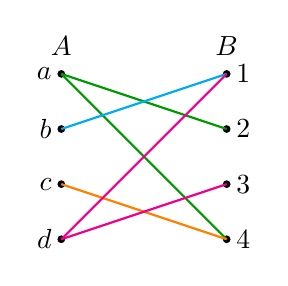
\begin{tikzpicture}[scale=0.7]
					
					\node at (0, 3.5) {$A$};
					\fill[black] (0, 3) circle (2pt) node[left] {$a$};
					\fill[black] (0, 2) circle (2pt) node[left] {$b$};
					\fill[black] (0, 1) circle (2pt) node[left] {$c$};
					\fill[black] (0, 0) circle (2pt) node[left] {$d$};
					
					\node at (3, 3.5) {$B$};
					\fill[black] (3, 3) circle (2pt) node[right] {$1$};
					\fill[black] (3, 2) circle (2pt) node[right] {$2$};
					\fill[black] (3, 1) circle (2pt) node[right] {$3$};
					\fill[black] (3, 0) circle (2pt) node[right] {$4$};
					
					\draw[green!60!black, thick] (0,3) -- (3,2);
					\draw[green!60!black, thick] (0,3) -- (3,0);
					\draw[cyan, thick] (0,2) -- (3,3);
					\draw[orange, thick] (0,1) -- (3,0);
					\draw[magenta, thick] (0,0) -- (3,3);
					\draw[magenta, thick] (0,0) -- (3,1);
				\end{tikzpicture}
				\caption{Grafo bipartito}
				
			\end{subfigure}
			\hfill
			\begin{subfigure}[c]{0.48\textwidth}
				
				\centering
				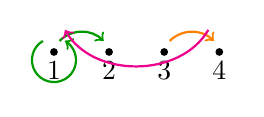
\begin{tikzpicture}[scale=0.7]
					\fill[black] (1, 0) circle (2pt) node[below] {$1$};
					\fill[black] (2, 0) circle (2pt) node[below] {$2$};
					\fill[black] (3, 0) circle (2pt) node[below] {$3$};
					\fill[black] (4, 0) circle (2pt) node[below] {$4$};
					
					\draw[green!60!black, thick, ->] (0.8, 0.2) arc (120:420:0.4);
					
					\draw[green!60!black, thick, ->] (1.1, 0.2) to[bend left=45] (1.9, 0.2);
					
					\draw[orange, thick, ->] (3.1, 0.2) to[bend left=45] (3.9, 0.2);
					
					\draw[magenta, thick, ->] (3.8, 0.4) to[bend left=60] (1.2, 0.4);
				\end{tikzpicture}
				\caption{Grafo diretto}
				
			\end{subfigure}
			
		\end{figure}
		
		Il grafo diretto si applica in caso di una relazione su un singolo insieme:
		\[
		R \subseteq B \times B = \{(1, 1), (1, 2), (3, 4), (4, 1)\}
		\]
		
		\item Si può usare una matrice con valori $0$ e $1$, valori che rappresentano rispettivamente l'assenza o la presenza di una coppia nella relazione.
		
		Usando sempre una relazione $R$ definita precedentemente:
		\[
		\begin{blockarray}{ccccc}
			& 1 & 2 & 3 & 4 \\
			\begin{block}{c(cccc)}
				a & 0 & 1 & 0 & 1 \\
				b & 1 & 0 & 0 & 0 \\
				c & 0 & 0 & 0 & 1 \\
				d & 1 & 0 & 1 & 0 \\
			\end{block}
		\end{blockarray}
		\]

	\end{itemize}
	
	\section{Relazione inversa}
	Come per le funzioni, anche per una relazione è possibile definirne l'inverso. A differenza delle funzioni, una relazione ha sempre un inverso.
	
	Sia $R \subseteq A \times B$, formato dalle coppie del tipo $(a, b)$. Definiamo $R^{-1} \subseteq B \times A$ formato dalle coppie $\{(b, a) : (a, b) \in R\}$.
	
	Nei grafi basta semplicemente invertire l'ordine delle frecce:
	\begin{center}
		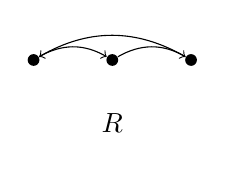
\begin{tikzpicture}
			\node[circle, fill, inner sep=1.5pt] (1) at (0,0) {};
			\node[circle, fill, inner sep=1.5pt] (2) at (1,0) {};
			\node[circle, fill, inner sep=1.5pt] (3) at (2,0) {};
			
			\draw[->, bend left] (1) to (2);
			\draw[->, bend left] (2) to (3);
			\draw[->, bend right] (3) to (1);
			
			\node at (1,-0.8) {$R$};
		\end{tikzpicture}
		\hspace{2cm}
		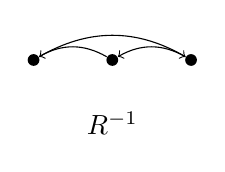
\begin{tikzpicture}
			\node[circle, fill, inner sep=1.5pt] (1) at (0,0) {};
			\node[circle, fill, inner sep=1.5pt] (2) at (1,0) {};
			\node[circle, fill, inner sep=1.5pt] (3) at (2,0) {};
			
			\draw[<-, bend left] (1) to (2);
			\draw[<-, bend left] (2) to (3);
			\draw[<-, bend right] (3) to (1);
			
			\node at (1,-0.8) {$R^{-1}$};
		\end{tikzpicture}
	\end{center}
	
	In una matrice notiamo un comportamento più interessante:
	\[
	M_R = \begin{pmatrix}
		1 & 1 & 1 \\
		0 & 1 & 0 \\
		0 & 0 & 1
	\end{pmatrix}
	\qquad
	M_{R^{-1}} = \begin{pmatrix}
		1 & 0 & 0 \\
		1 & 1 & 0 \\
		1 & 0 & 1
	\end{pmatrix}
	\]
	
	Si dice che $M_{R^{-1}}$ è la \textbf{trasposta} di $M_R$ in quanto, come vediamo:
	\begin{itemize}
		\item $1^a \text{ riga} \longrightarrow 1^a \text{ colonna}$
		\item $2^a \text{ riga} \longrightarrow 2^a \text{ colonna}$
		\item[$\vdots$]
		\item $n^a \text{ riga} \longrightarrow n^a \text{ colonna}$
	\end{itemize}
	
	\section{Composizione di relazioni}
	
	Siano $R \subseteq A \times B$ e $S \subseteq B \times C$. La \textbf{relazione composta} (o composizione) di $R$ e $S$ è la relazione che sussiste tra $a \in A$ e $c \in C$ se e solo se esiste $b \in B$ tale che $(a, b) \in R$ e $(b, c) \in S$.
	Viene indicata come $(S \circ R)$ (dove $R$ è quella che si applica prima).
	
	Facciamo un esempio esplicito:
	\begin{itemize}
		\item $R = \{(a, b), (b, b), (b, d), (c, a), (d, a)\}$
		\item $S = \{(a, d), (a, b), (b, c), (d, b)\}$
	\end{itemize}
	
	Allora dobbiamo prendere il secondo elemento di ogni tupla di $R$ e cercare una tupla in $S$ che inizia con quell'elemento. Prendendo poi il secondo elemento della coppia corrispondente in $S$, avremo creato $S \circ R$:
	\begin{itemize}
		\item per $(a, b)$, quelli in $S$ che iniziano con $b$ sono solo $(b, c)$ e dunque abbiamo $(a, c) \in (S \circ R)$
		\item così via per ogni elemento di $R$.
	\end{itemize}
	
	Nel caso di come abbiamo definito noi gli insiemi sopra, però, non esiste $(R \circ S)$ in quanto abbiamo $S \subseteq B \times C$, $R \subseteq A \times B$ e come vediamo $C \neq A$.
	
	\section{Proprietà delle relazioni}
	
	\begin{definizione}{Transitività}{}
		Una relazione $R \subseteq A \times A$ è detta \textbf{transitiva} se $\forall a, b, c \in A$, se $(a, b) \in R$ e $(b, c) \in R$, allora $(a, c) \in R$.
	\end{definizione}
	
	Per dimostrare che una relazione non è transitiva, ci basta trovare anche un solo controesempio (dato che nella definizione viene detto "per ogni").
	
	Prendiamo per esempio il seguente grafo:
	
	\begin{center}
		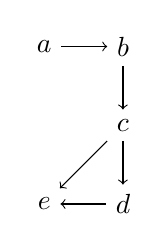
\begin{tikzpicture}
			\node (a) at (0, 1) {$a$};
			\node (b) at (1, 1) {$b$};
			\node (c) at (1, 0) {$c$};
			\node (d) at (1, -1) {$d$};
			\node (e) at (0, -1) {$e$};
			
			\draw[->] (a) -- (b);
			\draw[->] (b) -- (c);
			\draw[->] (c) -- (d);
			\draw[->] (d) -- (e);
			\draw[->] (c) -- (e);
		\end{tikzpicture}
	\end{center}
	
	Nonostante possa sembrare transitiva in quanto $(c, d) \in R$, $(d, e) \in R$ e $(c, e) \in R$, questo non vale per tutte le triple di valori in quanto $(a, b) \in R$ e $(b, c) \in R$ ma $(a, c) \notin R$, quindi non è transitiva.
	
	Inoltre, nella definizione di transitività non abbiamo posto vincoli su $a, b, c$, dunque questi potrebbero anche essere uguali. 
	Prendiamo un altro esempio: $a$ e $b$ collegati in entrambe le direzioni, ovvero $(a, b) \in R$, $(b, a) \in R$ ma $(a, a) \notin R$.
	
	Proviamo a renderla transitiva:
	\begin{itemize}
		\item Aggiungiamo l'autoarco su $a$. Ma di nuovo, se io scrivo $(b, a) \in R$ e $(a, b) \in R$, otteniamo che $(b, b) \notin R$.
		\item Aggiungiamo l'autoarco su $b$.
	\end{itemize}
	
	E stavolta, in quanto abbiamo stabilito tutti i collegamenti possibili, la relazione è transitiva.
	
	Vediamo altri due esempi particolari:
	Consideriamo una relazione i cui elementi sono definiti dai collegamenti tra $1 \to 2$, $1 \to 3$, $4 \to 2$, $4 \to 5$ e $6 \to 5$. Sarà transitiva? Non sembra.
	
	Cerchiamo un controesempio:
	\begin{itemize}
		\item $(1, 2) \in R$, ma $2$ non è collegato a nessuno, quindi non è un $b$ valido dato che non ha corrispondenze.
		\item $(4, 5) \in R$, stesso discorso del $2$ ma stavolta per il $5$.
	\end{itemize}
	
	Insomma, non importa quanto ci sforziamo a trovare un controesempio, non lo troveremo mai.
	Per questo motivo, dato che non riusciamo a dimostrare che $R$ non è transitiva, allora lo è e si dice \textbf{transitiva a vuoto}.
	
	\begin{definizione}{Chiusura transitiva}{}
		Chiamiamo \textbf{chiusura transitiva} di $R$ la più piccola relazione transitiva che estende $R$, ossia la relazione $R^T$ tale che:
		\begin{enumerate}
			\item $R \subseteq R^T$
			\item $R^T$ è transitiva
			\item Se $S$ estende $R$ ed è transitiva, allora $R^T \subseteq S$.
		\end{enumerate}
		Il terzo punto vale anche per insiemi infiniti!
	\end{definizione}
	
	\textbf{Esempio:} $R \subseteq A \times A$, $A = \N$. $R^T = \bigcup_{n \ge 0} R^n$.
	
	Definiamo la relazione $<$ come insieme delle coppie $(x, y)$ tale che $x < y$ oppure scrivibile come $y = x + n$, con $n > 0$.
	\[
	R^n = \{(x, y) \mid y = x + n, \, n > 0\} \longleftarrow \text{struttura generale di una $n$-esima relazione}
	\]
	
	Definiamo poi $<\, = \bigcup R^n$. Siccome stiamo facendo l'unione di relazioni infinite, ognuna transitiva, anche $<$ sarà transitiva.
	
	Possiamo dire che $(x, y) \in \bigcup R^n$ se e solo se $\exists n_1$ tale che $(x, y) \in R^{n_1}$.
	Una coppia di valori, per essere presente nell'unione delle relazioni, deve essere presente in almeno una delle relazioni dell'unione.
	
	\begin{definizione}{Riflessività}{}
		
		$R \subseteq A \times A$ è \textbf{riflessiva} se e solo se $\forall a \in A, \, (a, a) \in R$.
		
	\end{definizione}
	
	\begin{definizione}{Simmetria}{}
		
		$R \subseteq A \times A$ è simmetrica se e solo se $\forall a, b \in A$, se $(a, b) \in R$ allora $(b, a) \in R$.
		Dato $a \longleftrightarrow b \longleftrightarrow c$, questa è simmetrica in quanto non abbiamo una freccia unidirezionale tra $a$ e $c$, quindi non esiste proprio il collegamento.
		
	\end{definizione}
	
	Possiamo di conseguenza definire il concetto di \textbf{chiusura riflessiva} (mettiamo gli autoarchi per ogni elemento della relazione) e di \textbf{chiusura simmetrica} (mettiamo frecce bidirezionali per ogni collegamento esistente).
	
	\begin{definizione}{Relazione di equivalenza}{}
		$R \subseteq A \times A$ è una relazione di equivalenza se e solo se:
		\begin{enumerate}
			\item $R$ è transitiva;
			\item $R$ è riflessiva;
			\item $R$ è simmetrica.
		\end{enumerate}
	\end{definizione}
	
	\begin{osservazione}{}{}
		Sia $R \subseteq \mathbb{Z} \times \mathbb{Z}$, $(a, b) \in R$ se e solo se $a - b$ è pari. Verifichiamo le proprietà:
		\begin{itemize}
			\item \textbf{Riflessività}: $\forall a \in \mathbb{Z}, \, (a, a) \in R$, $a - a = 0$ che è sempre pari, dunque è \textbf{vero}.
			\item \textbf{Simmetria}: $\forall a, b \in \mathbb{Z}$, se $(a, b) \in R$ ($a - b$ pari) allora $(b, a) \in R$ ($b - a$ pari). Se uno dei due è pari lo sarà anche l'altro, ma con il segno cambiato.
			\item \textbf{Transitività}: $\forall a, b, c \in \mathbb{Z}$, se $(a, b) \in R$ e $(b, c) \in R$, allora $a - c = (a - b) + (b - c)$, che è somma di due quantità pari ed è quindi pari.
		\end{itemize}
	\end{osservazione}
	
	Supponiamo ora di avere un insieme $A = \N \times \N$ e una relazione $R \subseteq A \times A$.
	Ogni elemento di $R$ sarà dunque una coppia di coppie del tipo $((a, b), (c, d))$ definita solo per valori t.c. $a + d = b + c$.
	
	\begin{description}
		\item [Riflessiva:] $\forall (a, b) \in A, \, ((a, b), (a, b)) \in R$. Vero! Per la condizione di definizione $a + b = b + a$.
		\item [Simmetrica:] $\forall (a, b), (c, d) \in A$, $((a, b), (c, d)) \in R$ e $((c, d), (a, b)) \in R$.
		Di nuovo vero per la condizione di definizione: nell'elemento a sinistra abbiamo $a + d = b + c$ e a destra $c + b = d + a$.
		\item [Transitiva:] $\forall (a, b), (c, d), (e, f) \in A$.
		Se $((a, b), (c, d)) \in R$ e $((c, d), (e, f)) \in R$, allora $a + d = b + c \implies a - b = c - d$, e $c + f = d + e \implies c - d = e - f$.
		Da cui $a - b = e - f \implies a + f = b + e$.
		E infatti $((a, b), (e, f)) \in R$. Vero!
	\end{description}
	
	\section{Classi di equivalenza}
	Sia $R \subseteq A \times A$ una relazione di equivalenza. Sia $a \in A$ un elemento di $A$.
	
	Chiamiamo $[a]_R$ la \textbf{classe di equivalenza di $a$ in $R$}, formalmente definita come:
	\[
	[a]_R = \{a' \in A : (a, a') \in R\}
	\]
	dunque sostanzialmente tutti gli elementi di $A$ che sono in relazione con $a$ tramite $R$.
	
	\begin{osservazione}{}{}
		Se $R$ è di equivalenza, sarà anche riflessiva e dunque vi sarà presente la coppia $(a, a)$ rendendo impossibile $[a]_R = \O$.
	\end{osservazione}
	
	Per una casistica del tipo $a \longleftrightarrow a'$ avremo $[a]_R = \{a, a'\}$ e $[a']_R = \{a', a\}$.
	
	Diciamo che $R$ è equivalente su $A$ se per ogni $a, a' \in A$
	\[
	[a]_R = [a']_R \quad \text{oppure} \quad [a]_R \cap [a']_R = \O
	\]
	% --- NEW PAGE ---
	
	Per quest'ultima dimostrazione possiamo vedere come due classi di equivalenza su un insieme $A$ tramite relazione $R$:
	\begin{itemize}
		\item sono uguali oppure
		\item sono disgiunte.
	\end{itemize}
	
	E questo ci porta a pensare che l'insieme delle classi $[a]_R$ forma una partizione dell'insieme $A$:
	\[
	A = \bigcup_{a \in A} [a]_R
	\]
	
	Vediamo però che possiamo fare anche il percorso inverso, cioè dalla partizione alla relazione equivalente.
	Supponiamo di avere la partizione $A = \bigcup_{i \in I} C_i$ con $C_i$ disgiunti.
	Definiamo $R \subseteq A \times A$ con $(a, b) \in R$ se e solo se $a, b \in C_i$.
	Se appartengono allo stesso sottoinsieme sono in relazione, altrimenti no.
	
	\section{Insiemi Quoziente}
	
	\begin{osservazione}{}{}
		Se ad una relazione $R$ che è transitiva e simmetrica aggiungiamo un punto isolato $c$, questa rimane transitiva e simmetrica.
	\end{osservazione}
	
	Tuttavia, se una relazione è transitiva e simmetrica, non è detto che sia anche riflessiva. Infatti, se consideriamo un elemento $c$ aggiunto che non ha un autoarco, la proprietà riflessiva viene a mancare.
	
	Supponiamo di avere $(a,b) \mathrel{R} (c,d)$ se e solo se $a + d = b + c$.
	
	Possono definire la classe d'equivalenza $[(a,b)]_R$ nel seguente modo:
	\[
	[(a,b)]_R = \{(c,d) \mid (a,b) \mathrel{R} (c,d)\} = \{(c,d) \mid a + d = b + c\} = \{(c,d) \mid a - b = c - d\}
	\]
	Questa definizione ci sta dicendo che tutte le coppie associate hanno la stessa differenza.
	
	Possiamo, con questo esempio, definire l'\textbf{insieme quoziente}.
	
	\begin{definizione}{Insieme quoziente}{}
		Sia $A$ un insieme e $R$ una relazione di equivalenza su quell'insieme, definiamo l'insieme quoziente come l'insieme delle classi di equivalenza di $A$:
		\[
		A/R = \{[a]_R \mid a \in A\}
		\]
	\end{definizione}
	
	Nel nostro caso specifico, ogni classe di equivalenza è identificata da un numero intero:
	\[
	A/R = \{C_k \mid k \in \Z\} \quad \text{dove} \quad C_k = \{(a,b) \mid a - b = k\}
	\]
	
	\section{Relazioni d'ordine}
	
	Generalizzazione della relazione $\le \subseteq \N \times \N$:
	\begin{enumerate}
		\item \textbf{Riflessiva}: $\forall a, \, a \le a$
		\item \textbf{Transitiva}: $\forall a, b, c$, se $a \le b$ e $b \le c$, allora $a \le c$
		\item \textbf{Simmetrica?} Se $a \le b$, $b \le a$? Assolutamente no! Si dice dunque gravemente non simmetrica oppure \textbf{antisimmetrica}.
		\item \textbf{Totalità}: Presi due numeri $a, b$ qualunque, questi sono sempre confrontabili.
	\end{enumerate}
	
	Grazie a questo esempio possiamo introdurre due concetti fondamentali:
	\begin{itemize}
		\item $R \subseteq A \times A$ è un \textbf{ordine totale} (o \textbf{lineare}) se possiede tutte e 4 le proprietà elencate prima (es: $\le$ visto sopra).
		\item $R \subseteq A \times A$ è un \textbf{ordine parziale} se possiede le prime 3 tra le proprietà elencate prima e viola la quarta.
	\end{itemize}
	
	\begin{osservazione}{}{}
		Prendiamo come esempio l'inclusione insiemistica $\subseteq$:
		\begin{enumerate}
			\item $S \subseteq S$: vero, riflessiva;
			\item $S \subseteq T$ e $T \subseteq Q \implies S \subseteq Q$: vero, transitiva;
			\item $S \subseteq T$ e $T \subseteq S \implies S = T$: vero, antisimmetrica;
			\item Usiamo un esempio numerico: $A = \{1\}, B = \{2\}$
			\begin{itemize}
				\item $A \subseteq B$? No.
				\item $B \subseteq A$? No.
			\end{itemize}
			E allora si dicono \textbf{inconfrontabili}.
		\end{enumerate}
	\end{osservazione}
	
	\begin{teorema}{Estensione totale}{}
		Ogni ordine parziale ammette un'\textbf{estensione totale}.\\
		Sia $R \subseteq A \times A$ una relazione di ordine parziale.\\
		Siano $a, b \in A$ due elementi incomparabili rispetto ad $R$ (ossia che $(a, b) \notin R$ e $(b, a) \notin R$, non sono collegati).\\
		Esiste una relazione $R' \subseteq A \times A$ tale che:
		\begin{enumerate}
			\item $R \subseteq R'$ ($R'$ estensione di $R$).
			\item $(a, b) \in R'$.
		\end{enumerate}
	\end{teorema}
	
	\begin{dimostrazione}{Dimostrazione}{}
		Definiamo $R'$ aggiungendo la coppia $(a, b)$ e tutte le coppie $(x, y)$ tali che $xRa$ e $bRj$.
		Stiamo considerando tutti gli elementi $x$ che stanno prima di $a$ secondo $R$ e tutti gli elementi $y$ che stanno dopo $b$ secondo $R$. In termini insiemistici:
		\[
		X = \{x \in A \mid xRa\} \qquad Y = \{y \in A \mid bRy\}
		\]
		La relazione $R'$ è definita dunque come $R \cup (X \times Y)$.
	\end{dimostrazione}
	
	\newpage
	In poche parole:
	\begin{itemize}
		\item $R' = R \cup \{(a, b)\}$, aggiungiamo la coppia $(a, b)$ che per definizione $\notin R$. Questo forza il fatto che $a$ e $b$ siano comparabili, ma potrebbe violare la transitività di $R'$ (ereditata da $R$).
		\item Definiamo $X = \{x \in A \mid xRa\}$ come "tutti gli elementi in $R$ che stanno sotto ad $a$", e $Y = \{y \in A \mid bRy\}$ come "tutti gli elementi in $R$ che stanno sopra a $b$".
		\item In $R'$ adesso abbiamo:
		\begin{itemize}
			\item $(x, a)$, già presenti in $R$;
			\item $(a, b)$, aggiunti poco fa;
			\item $(b, y)$, già presenti in $R$.
		\end{itemize}
		Notiamo che, per preservare la transitività, ci manca la coppia $(x, y)$ che dunque aggiungiamo.
		\item Risultato: $R' := R \cup (X \times Y)$
	\end{itemize}
	
	Costruito $R'$, verifichiamo se sia o meno un ordine totale:
	\begin{itemize}
		\item È transitiva, e ce ne siamo occupati prima;
		\item È riflessiva perché $R$ era riflessiva;
		\item Antisimmetrica? Sì!
		
		Supponiamo sia simmetrica e dunque $x R' y$ e $y R' x$. Per come è definita $R'$, abbiamo vari casi:
		\begin{itemize}
			\item \textbf{Caso 1:} $(x, y) \in X \times Y$ e $(y, x) \in X \times Y$ allora $x \in X \cap Y$, ma questo è impossibile dato che $X \cap Y = \emptyset$. Se fosse $z \in X \cap Y$ allora $z \in X$, $zRa$ e $z \in Y$, $b Rz$. Ma dato che $R$ è transitiva dovremmo avere $bRa$ ma ciò contraddice l'ipotesi che $a$ e $b$ fossero incomparabili.
			\item \textbf{Caso 2:} $(x, y) \in X \times Y$ e $(y, x) \in R'$ allora $(x, a) \in R$ ma per transitività di $R$ dovremmo avere anche $yRa$. Ma $y \in Y$ e dunque $bRy$. Si crea nuovamente la situazione di prima per cui dovremmo avere $bRa$ ma non possiamo in quanto sono incomparabili.
			\item \textbf{Caso 3:} $(y, x) \in X \times Y$ e $(x, y) \in R'$, dimostrazione analoga al caso precedente.
		\end{itemize}
		
		\item Totale, in quanto tutte le coppie incomparabili sono state risolte dall'aggiunta di $X \times Y$ che comprende gli elementi sotto a $a$ e sopra a $b$.
	\end{itemize}
	
	\section{Cicli}
	
	Sia $R$ un ordine parziale su un insieme $A$. Allora $R$ non ha cicli eccetto quelli di tipo $aRa$ dati dalla sua riflessività.
	
	Per ciclo intendiamo un percorso che inizia e finisce nello stesso punto, ossia $a_1 R a_2 R \dots R a_m R a_1$ con $a_1, \dots, a_n$ tutti distinti. La lunghezza del ciclo è il numero di archi (ossia di relazioni $R$).
	
	\begin{dimostrazione}{}{}
		Supponiamo di avere un ciclo $a_1 R a_2 R \dots R a_m R a_1$ su una relazione parziale $R$. Per transitività di $R$ abbiamo che $a_1 R a_2 R a_3$ implica $a_1 R a_3$, e analogamente $a_1 R a_3 R a_4$ implica $a_1 R a_4$.
		In generale quindi $a_1 R a_m$ e $a_m R a_1$. Ma per antisimmetria di $R$ ciò è possibile solo per $a_1 = a_m$.
	\end{dimostrazione}
	
	\section{Elementi minimali}
	
	Ogni ordine parziale contiene almeno un minimale, cioè un elemento che non è preceduto da nessun altro (non arrivano frecce, partono solo). Formalmente:
	\[
	R \subseteq A \times A \text{ parziale}, \quad a \in A \text{ è minimale se } \forall b \in A \setminus \{a\} \text{ non vale } bRa
	\]
	
	\begin{dimostrazione}{}{}
		Consideriamo un cammino di lunghezza massima in $A$, ossia una scelta di elementi $a_1, \dots, a_m$ t.c. $a_1 R a_2 R \dots R a_{m-1} R a_m$ e non esista un cammino di lunghezza maggiore.
		
		Si nota facilmente che se prendendo un $a \in A$ diverso da tutti gli $a_1, \dots, a_m$ significa che è un nuovo elemento e staremo dunque contraddicendo l'ipotesi della lunghezza massima.
		
		Se invece poniamo un nuovo $a = a_i$, con $a_i$ un qualsiasi elemento del cammino e $a R a_i$ allora si formerebbe un ciclo di lunghezza $i$ che contraddirebbe l'ipotesi di $R$ ordine parziale.
	\end{dimostrazione}
	
	Un minimo di un ordine parziale è quel valore che viene succeduto da tutti gli elementi di $A$ in $R$.
	\[
	m \text{ è minimo se } \forall x \in A \text{ vale } mRx
	\]
	
	Dunque un minimo è anche un minimale ma non si può affermare con certezza il contrario.
	
	\chapter{Induzione}
	
	Prima di provare a dimostrare l'estensibilità totale di una relazione $R$ con il principio di induzione, andiamo a vedere quale è la struttura di una dimostrazione induttiva.
	
	\section{Struttura del principio induttivo}
	Vogliamo stabilire una tesi universale, ossia che per ogni $n \geq 1$ vale una certa proprietà $P(n)$.
	È sufficiente dimostrare i due punti seguenti:
	\begin{enumerate}
		\item \textbf{Base}: verifichiamo/dimostriamo che la proprietà vale per $n = 1$.
		\item \textbf{Passo induttivo}: considerando un generico $n \geq 1$, assumiamo che la proprietà valga per $n$ (ipotesi induttiva) e dimostriamola dunque per $n+1$. Ossia dimostriamo che vale l'implicazione: se $P(n)$ allora $P(n+1)$, ovvero $P(n) \implies P(n+1)$.
	\end{enumerate}
	
	Poste le dovute basi, possiamo ora procedere con la dimostrazione anticipata nella premessa.
	
	\begin{description}
		
		\item [Tesi]: Per ogni possibile cardinalità $n$, per ogni insieme $A$ di cardinalità $n$, per ogni ordine parziale $R$ su $A$, esiste un ordine totale $R^*$ su $A$ tale che $R \subseteq R^*$.
		
		\item [Caso base ($n=1$)]: Consideriamo un insieme $A = \{a\}$. L'unico ordine parziale $R$ su $A$ è di tipo $R = \{(a, a)\}$, che è un ordine anche totale. La tesi è verificata: l'estensione totale di $R$ è $R$ stesso.
		
		\item [Passo induttivo]: Assumiamo la tesi sia vera fino ad un certo $n$ e proviamo dunque per $n+1$.
		
	\end{description}
	
	Sia $A$ un insieme di $n+1$ elementi. Come osservato precedentemente, esiste almeno un elemento $a \in A$ che è minimale. Dunque, l'insieme $A \setminus \{a\}$ ha $n$ elementi. Inoltre, la relazione $R^-$ su $A \setminus \{a\}$ ottenuta cancellando da $R$ tutte le coppie che contengono $a$ è un ordine parziale.
	
	Per l'ipotesi induttiva abbiamo assunto di saper dimostrare la tesi per insiemi di cardinalità $n$. In particolare possiamo farlo per l'ordine $R^-$ definito prima. Esiste dunque un ordine totale $R_T^-$ su $A \setminus \{a\}$, $R^- \subseteq R_T^-$.
	
	Esiste dunque un ordine $R_T$ su $A$ definito come segue:
	\[
	R_T = R_T^- \cup \{(a, x) \colon a \in A\}
	\]
	e facilmente si dimostra che è un ordine totale.
	
	La tesi è del tutto verificata.
	
	Ci si potrebbe chiedere perché il principio di induzione funzioni. Ossia, perché se $P(1)$ è vera e $P(n) \implies P(n+1)$, allora $P(n)$ è vera $\forall n \ge 1$?
	
	\textbf{Strutturalmente:} conoscendo la struttura dei numeri naturali, sappiamo che, partendo da $0$, ogni numero equivale al precedente più $1$. Dunque, se una proprietà viene passata ad esempio da $1$ a $2$, significa che la somma di una singola unità preserva la proprietà. Se ciò vale per $1$ e $2$, allora vale anche per un generico numero $n$ ed il suo successivo $n+1$.
	
	\begin{dimostrazione}{Dimostrazione per assurdo del principio di induzione}{}
		Supponiamo che $P(1)$ sia vera e che $\forall n \ge 1$ si abbia $P(n) \implies P(n+1)$, ma che non valga $P(n)$ per ogni $n \ge 1$.
		Dunque, per assurdo, esiste almeno un valore per cui non vale $P(n)$.
		Costruiamo $C$ come l'insieme di tutti i valori $n \in \N$ per cui non vale $P(n)$:
		\[
		C = \{n \in \N \mid n \ge 1 \text{ e } \neg P(n)\} \neq \O
		\]
		L'insieme $C$ è dunque un sottoinsieme di $\N$ e, per definizione, ha un minimo, che chiamiamo $n_0$.
		Ora analizziamo i possibili valori di $n_0$:
		\begin{itemize}
			\item Se $n_0 = 1$, ciò è assurdo perché sappiamo per ipotesi che $P(1)$ è vera.
			\item Allora $n_0 > 1$, ma siccome siamo nei naturali possiamo dire analogamente che $n_0 - 1 \ge 1$.
		\end{itemize}
		Siccome $n_0$ è il minimo numero per cui $P(n)$ è falsa, $P(n_0 - 1)$ è per forza vera.
		Seguendo lo schema induttivo, da $P(n_0 - 1)$ discende $P(n_0)$, ma per definizione di $C$ sappiamo invece che $P(n_0)$ è falsa.
		Abbiamo così ottenuto una contraddizione, il che conclude la dimostrazione.
	\end{dimostrazione}
	
	Vediamo come applicare questo principio attraverso un esempio classico.
	
	\begin{osservazione}{Dimostrazione per induzione della formula di Gauss}{}
		Gauss ha sviluppato una formula per calcolare la somma dei primi $n$ numeri naturali:
		\[
		1 + 2 + 3 + \dots + n = \frac{n(n+1)}{2}
		\]
		In questo caso la nostra proprietà $P(n)$ è proprio l'identità stessa.
		\begin{itemize}
			\item \textbf{Caso base}: per $n = 1$, abbiamo $1 = \frac{1(1+1)}{2}$, che è ovviamente vera.
			\item \textbf{Ipotesi induttiva}: assumiamo $P(n)$ vera.
			\item \textbf{Passo induttivo}: vogliamo dimostrare $P(n+1)$.
		\end{itemize}
		Scriviamo la somma per $n+1$:
		\[
		P(n+1) = \underbrace{1 + 2 + \dots + n}_{\text{riconosciamo } P(n) \text{ qui dentro}} + (n+1) = \frac{(n+1)(n+2)}{2}
		\]
		Sostituendo l'ipotesi induttiva otteniamo:
		\[
		\frac{n(n+1)}{2} + (n+1) = \frac{(n+1)(n+2)}{2}
		\]
		Facendo qualche calcolo puramente algebrico vediamo che l'uguaglianza è verificata e dunque la tesi è dimostrata.
	\end{osservazione}
	
	L'induzione può anche essere applicata anche per dimostrare conteggi combinatori.
	
	\begin{dimostrazione}{Numero di sottoinsiemi di un insieme di $n$ elementi}{}
		Vogliamo dimostrare che il numero di sottoinsiemi di un insieme di $n$ elementi è $2^n$.
		
		\textbf{Base}: $n = 1$. Sia $A = \{a_1\}$. Come possiamo vedere, $A$ ha $2$ sottoinsiemi: $\mathcal{P}(A) = \{\emptyset, \{a_1\}\}$.
		
		\textbf{Passo induttivo}: Sia $A$ un insieme di $n+1$ elementi: $A = \{a_1, a_2, \dots, a_n, a_{n+1}\}$. Fissiamo l'elemento $a_1$.
		I sottoinsiemi $S$ di $A$ possono essere di due tipi:
		\begin{itemize}
			\item $a_1 \in S$ del tipo $S = \{a_1\} \cup S^*$ con $S^* \subseteq A \setminus \{a_1\}$. Anche qui $S^*$ è un insieme di $n$ elementi e dunque per ipotesi induttiva abbiamo $2^n$ possibilità.
			\item $a_1 \notin S$ del tipo in cui $S \subseteq A \setminus \{a_1\}$. Anche in questo caso, trattandosi di sottoinsiemi di un insieme di $n$ elementi, per ipotesi induttiva abbiamo altri $2^n$ sottoinsiemi.
		\end{itemize}
		Sommando i due contributi otteniamo:
		\[
		2^n + 2^n = 2 \cdot 2^n = 2^{n+1}
		\]
		La dimostrazione è così conclusa.
	\end{dimostrazione}
	
	\begin{osservazione}{}{}
		Siano $A$ e $B$ due insiemi tali che $\#A = \#B = n$. Allora tra i due insiemi esistono $n!$ biezioni possibili.
	\end{osservazione}
	
	Dimostriamo questa proprietà per induzione.
	\begin{dimostrazione}{Dimostrazione per induzione}{}
		\begin{itemize}
			\item \textbf{Base}: se $n = 1$, siano $A = \{a\}$ e $B = \{b\}$. L'unica biezione possibile è $a \mapsto b$, che corrisponde esattamente a $n! = 1! = 1$.
			\item \textbf{Passo induttivo}: supponiamo che la proprietà valga per $n$ e dimostriamola per $n+1$. Siano $A = \{a_1, a_2, \dots, a_n, a_{n+1}\}$ e $B = \{b_1, b_2, \dots, b_n, b_{n+1}\}$. Fissiamo $a_{n+1} \mapsto b_{n+1}$ e consideriamo i sottoinsiemi $A \setminus \{a_{n+1}\}$ e $B \setminus \{b_{n+1}\}$. Rimangono dunque due insiemi con $n$ elementi per cui vale l'ipotesi induttiva. Considerando $a_{n+1}$ e $b_{n+1}$ rimossi, abbiamo adesso che $a_{n+1}$ può avere $n+1$ immagini in $B$. Dunque per ogni valore di $f(a_{n+1})$ ci sono $n!$ possibili associazioni, e ciò vale per ciascuno degli $n+1$ elementi di $B$.
		\end{itemize}
	\end{dimostrazione}
	
	\section{Problema dei piastrellamenti}
	
	Consideriamo il seguente problema: abbiamo un pavimento quadrato composto di $2^n \times 2^n$ quadrati. Vogliamo ricoprirlo di piastrelle bianche a forma di $L$, lasciando spazio libero in una delle posizioni centrali del pavimento per una piastrella nera.
	
	Proviamo a dimostrare per induzione che è possibile farlo $\forall n \geq 1$.
	
	\begin{itemize}
		\item \textbf{Caso base}: se ho un pavimento $2^1 \times 2^1$ allora ho addirittura $4$ modi di lasciare libera una piastrella centrale (anche perché nell'ipotesi minima sono tutte centrali).
	\end{itemize}
	
	Assumiamo di saper pavimentare ogni pavimento di lato $2^n$ e dimostriamo dunque di saperlo fare anche per il lato $2^{n+1}$.
	
	Matematicamente $2^{n+1} = 2 \cdot 2^n$, e dunque possiamo scomporre il nostro pavimento in $4$ quadrati di lato $2^n$.
	
	Da ciò, per ipotesi induttiva, sappiamo che per un quadrato di lato $2^n$ possiamo disporre le piastrelle in modo da lasciare uno spazio libero al centro del quadrato.
	
	Come vediamo, però, questo non ci aiuta affatto nel dimostrare il caso $n+1$.
	
	Quindi? Ci arrendiamo?
	
	Non ancora.
	
	Riguardando il caso base ci rendiamo conto che questo permette di lasciare una piastrella vuota al centro, bensì in un punto qualsiasi del quadrato.
	
	E questa è chiaramente un'ipotesi induttiva molto più forte della precedente.
	
	Proviamo ora a dimostrare il caso $n+1$ con questa nuova ipotesi:
	
	\begin{center}
		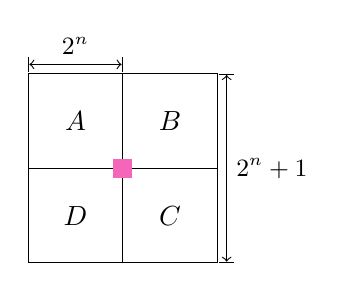
\begin{tikzpicture}[scale=1.2]
			\draw (0,0) rectangle (2,2);
			\draw (1,0) -- (1,2);
			\draw (0,1) -- (2,1);
			
			\node at (0.5, 1.5) {$A$};
			\node at (1.5, 1.5) {$B$};
			\node at (0.5, 0.5) {$D$};
			\node at (1.5, 0.5) {$C$};
			
			\draw[|<->|] (0, 2.1) -- (1, 2.1) node[midway, above] {\small $2^n$};
			\draw[|<->|] (2.1, 0) -- (2.1, 2) node[midway, right] {\small $2^n+1$};
			
			\fill[magenta!60] (0.9, 0.9) rectangle (1.1, 1.1);
		\end{tikzpicture}
	\end{center}
	
	E casualmente noi sceglieremo come piastrelle libere proprio quelle che formano un quadrato $1 \times 1$ al centro del pavimento $2^{n+1} \times 2^{n+1}$.
	
	Perché ciò è vantaggioso?
	
	Semplicemente perché ora nel quadrato colorato riconosciamo il caso base, per il quale sappiamo che possiamo disporre una piastrella in qualsiasi modo, e che sempre avremo uno spazio libero.
	
	Siamo dunque partiti da $P(n) =$ ogni pavimento $2^n \times 2^n$ si può ricoprire con piastrelle a $L$ lasciando libera una posizione centrale e l'abbiamo rafforzata con $Q(n) =$ ogni pavimento $2^n \times 2^n$ si può ricoprire con piastrelle a $L$ lasciando libera una qualsiasi posizione.
	
	Siccome $Q$ è più forte di $P$, possiamo dire che $Q(n)$ implica $P(n)$.
	
	Nel nostro caso specifico, inoltre, è stato grazie a $Q(n)$ se siamo riusciti a dimostrare $P(n+1)$.
	
	Si noti però che, dal fatto che è vera $Q(1)$, e che $\forall n \ge 1$ abbiamo stabilito l'implicazione $Q(n) \to P(n+1)$, non possiamo concludere usando l'induzione che $\forall n \ge 1$ vale $P(n)$.
	Abbiamo stabilito i seguenti fatti:
	\[
	Q(1), Q(1) \to P(2), Q(2) \to P(3), \dots
	\]
	ma questa catena di implicazioni non ci permette di concludere che per ogni $n \ge 1$ vale $P(n)$.
	
	Per questo motivo abbiamo dovuto dimostrare, per $n \ge 1$, l'implicazione $Q(n) \to Q(n+1)$ e non $Q(n) \to P(n+1)$.
	
	\begin{dimostrazione}{Dimostrazione del secolo}{}
		Dimostriamo per induzione che tutti i credenti credono nello stesso Dio.
		
		Sia $D$ un Dio e $C$ l'insieme dei credenti.
		\begin{itemize}
			\item \textbf{Base}: $n = 1,\, C = \{c_1\}$ (dove $c_1$ crede in un solo $D$).
			\item \textbf{Passo}: $n + 1,\, C = \{c_1, c_2, \dots, c_n, c_{n+1}\}$ dove non è detto che tutti credano nello stesso.
		\end{itemize}
		Sia $A = C \setminus \{c_1\} = \{c_2, \dots, c_{n+1}\}$ di $n$ elementi, quindi per il passo induttivo vale $P(n)$.
		Sia $B = C \setminus \{c_{n+1}\} = \{c_1, c_2, \dots, c_n\}$, vale $P(n)$.
		
		Notiamo che $c_2 \in A \cap B$, e dato che $c_2$ crede in un solo Dio, allora facendo parte $A, B \subseteq C$ allora tutti in $C$ credono in un solo Dio.
	\end{dimostrazione}
	
	Per quanto possa essere fantastico il precedente esempio, in quanto ci permetterebbe di risolvere molti conflitti in corso, la tesi è chiaramente falsa e la dimostrazione presenta un problema non irrilevante:
	
	\begin{itemize}
		\item Dopo aver calcolato il caso base $n = 1$ abbiamo subito assunto $P(n)$ e provato a dimostrare $P(n+1)$.
		\item Non ci siamo neanche soffermati sui casi intermedi, come $P(2)$:
		\[
		C = \{c_1, c_2\}, \quad C_1 = \{c_1\}, \quad C_2 = \{c_2\}
		\]
		Come vediamo, non possiamo usare il metodo dimostrativo che avevamo usato per $P(n)$ in quanto $C_1 \cap C_2 = \emptyset$.
		E non possiamo neanche partire da $P(3)$ siccome l'implicazione $P(2) \to P(3)$ è falsa in quanto $P(2)$ è falsa.
		\item Per $n = 3, 4, 5, \dots$ la proprietà è valida! Peccato che $P(2)$ sia falsa e dunque si spezzi "un anello della catena", non rendendo più valida l'implicazione $\forall n \ge 1, \, P(n) \to P(n+1)$.
	\end{itemize}
	
	Abbiamo dunque denotato uno dei limiti del principio di induzione "classico".
	
	\section{Principio di induzione forte}
	
	\begin{teorema}{}{}
		Ogni numero naturale $\ge 2$ può scriversi come prodotto di numeri primi.
	\end{teorema}
	
	Proviamo a dimostrarlo per induzione:
	\begin{itemize}
		\item \textbf{Base}: $n = 2, \, 2 = 2 \cdot 1$ \checkmark
		\item \textbf{Passo}: Per la nostra ipotesi $n = p_1 \cdot p_2 \cdot \dots \cdot p_k$. Dobbiamo dedurre che $n + 1 = p_1 \cdot p_2 \cdot \dots \cdot p_k + 1$.
	\end{itemize}
	
	Il che non è affatto semplice. Proviamo un altro approccio:
	Per assurdo, supponiamo la tesi sia falsa. Definiamo:
	\[
	C = \{n : n \ge 2 \text{ e non è fattorizzabile in primi}\} \neq \emptyset
	\]
	Siccome $C \subseteq \N$ allora $\exists m = \min(C)$, che ovviamente non è primo altrimenti non sarebbe in $C$.
	
	Possiamo dunque riscrivere $m = a \cdot b$ e $2 \le a, b < m$.
	
	Dato che $a, b < m$ allora $a, b \notin C$. Inoltre dato che $2 \le a \cdot b$, il motivo per cui $a, b \notin C$ è che posseggono una scomposizione in primi.
	
	Possiamo dunque riscrivere $a = p_1 \cdot \dots \cdot p_k$, $b = q_1 \cdot \dots \cdot q_k$.\\
	Ma se $m = a \cdot b = p_1 \cdot \dots \cdot p_k \cdot q_1 \cdot \dots \cdot q_k$ allora ammette una fattorizzazione in primi. Contraddizione a MEC!
	
	Nell'argomento di sopra ci siamo ritrovati a ragionare su due elementi più piccoli del minimo dei controesempi, dunque non ci siamo limitati solo al caso base e $n+1$.
	
	\begin{definizione}{Principio di induzione forte}{}
		Sia $P$ una proprietà di $n \in \N$ e $k \in \N$. Se valgono i seguenti punti:
		\begin{enumerate}
			\item \textbf{(Base)} Vale $P(k)$ ($k$ è detta base).
			\item \textbf{(Passo)} $\forall n \ge k$, se $P(k), P(k+1), \dots, P(n)$ allora $P(n+1)$.
		\end{enumerate}
		allora posso concludere che $\forall n \ge k, \, P(n)$.
	\end{definizione}
	
	Sempre mediante il principio di induzione forte proviamo a dimostrare la sequenza di Fibonacci.
	
	La successione di Fibonacci è definita come:
	\begin{itemize}
		\item $F_0 = 0$
		\item $F_1 = 1$
		\item $F_n = F_{n-1} + F_{n-2}$, per $n \ge 2$
	\end{itemize}
	
	La nostra tesi è la seguente: $\forall n \ge 1, \, F(n) \le 2^n$.
	\begin{itemize}
		\item \textbf{Caso base}: $n = 1 \implies F(1) = 1$, $1 \le 2^1$.
		\item \textbf{Passo}:
		Tesi: Sia $n \ge 1$, $F_{n+1} \le 2^{n+1}$.
	\end{itemize}
	\[
	F(n+1) = F_n + F_{n-1}
	\]
	Per ipotesi induttiva sappiamo che $F_n \le 2^n$ e dunque sicuramente, dato che $F_{n-1} \le F_n \le 2^n \le 2^{n+1}$, allora $F_{n-1} \le 2^{n+1}$.
	
	A livello di logica induttiva funziona tutto.
	
	Proviamo però degli esempi numerici:
	\begin{itemize}
		\item Primo valore: $n=1$, $n+1=2$.
	\end{itemize}
	
	\[
	F_{n+1} = F_n + F_{n-1} \implies F_2 = F_1 + F_0
	\]
	
	Per $F_1$ abbiamo già dimostrato con il caso base che $F_1 < 2^1$.
	Tuttavia per $F_0$ non abbiamo dimostrato nulla, dunque la dimostrazione applicata per il caso $n+1$ non vale qui.
	
	Come facciamo? Semplice! Basta dimostrare un altro caso base, che nel nostro caso sarà $F_2$ (dato che $n=0 < 1$ e dunque è fuori dal range induttivo) e che sarà semplice e concluderà la dimostrazione.
	
	Stavolta proviamo a dimostrare che $\forall n \ge 2, \, F(n) \ge \left(\frac{3}{2}\right)^{n-2}$.
	
	\begin{itemize}
		\item \textbf{Caso base}: $n=2$, $F(2) \ge \left(\frac{3}{2}\right)^{2-2} \implies 1 \ge 1$.
		\item \textbf{Passo}: Sia $n \ge 2$.
	\end{itemize}
	
	\[
	F(n+1) \ge \left(\frac{3}{2}\right)^{(n+1)-2} \implies F_n + F_{n-1} \ge \left(\frac{3}{2}\right)^{n-1}
	\]
	
	Sempre per ipotesi induttiva sappiamo che:
	\[
	F_n \ge \left(\frac{3}{2}\right)^{n-2}, \quad F_{n-1} \ge \left(\frac{3}{2}\right)^{n-3}
	\]
	
	E anche stavolta, siccome abbiamo $n-3$, per il caso $n=2$ andiamo in una casistica \textit{out-of-range}.
	Dimostriamo semplicemente il caso per $n=3$ e, in quanto questo sarà diventato un caso base, nel nostro passo dovremmo scrivere $n \ge 3$.
	
	Provando poi ad applicare il caso per $n+1=4$, questo richiederà $F_3$ ed $F_2$, che sono entrambi casi base già dimostrati.
	
	\begin{dimostrazione}{Dimostrazione della proprietà di Fibonacci}{}
		\textbf{Caso base ($n=1$):} dobbiamo sommare tutti i termini di indice pari a partire da $0$ fino ad arrivare a $2n = 2\cdot 1 = 2$.
		Valutiamo separatamente i due membri dell'uguaglianza:
		\begin{itemize}
			\item $F_0 + F_2 = 0 + 1 = 1$
			\item $F_{2\cdot 1 + 1} - 1 = F_3 - 1 = F_2 + F_1 - 1 = 1 + 1 - 1 = 1$
		\end{itemize}
		Il caso base è così verificato, poiché i due membri coincidono.
		
		\textbf{Passo induttivo ($n \ge 1$):} assumiamo che la proprietà $P(n)$ sia vera e dimostriamo che vale $P(n+1)$.
		Possiamo riscrivere la sommatoria per il passo successivo in due modi equivalenti:
		\begin{itemize}
			\item $F_0 + F_2 + \dots + F_{2n} + F_{2n+2}$
			\item $\sum_{i=0}^{n+1} F_{2i}$
		\end{itemize}
		Sfruttiamo la prima forma per scomporre l'espressione e riconoscere l'ipotesi induttiva:
		\[
		\underbrace{F_0 + F_2 + \dots + F_{2n}}_{\text{vale l'ipotesi induttiva } = F_{2n+1} - 1} + F_{2n+2} = F_{2n+1} - 1 + F_{2n+2}
		\]
		Ci rendiamo conto che la somma $F_{2n+1} + F_{2n+2}$ non è altro che la somma di due termini consecutivi della successione di Fibonacci, la quale genera il termine successivo $F_{2n+3}$.
		Possiamo dunque riscrivere tale termine come $F_{2n+3} = F_{2(n+1)+1}$. Sostituendo nella precedente identità otteniamo:
		\[
		F_0 + F_2 + \dots + F_{2n} + F_{2n+2} = F_{2(n+1)+1} - 1
		\]
		che è esattamente la formula di partenza applicata al caso $(n+1)$-esimo. La dimostrazione è così conclusa.
	\end{dimostrazione}
	
	Estendiamo ora il metodo per dimostrare proprietà relative a successioni definite per ricorrenza.
	
	Consideriamo la successione definita per ricorrenza in questo modo:
	\[
	\begin{cases}
		a_1 = 2 \\
		a_2 = 3 \\
		a_{n+2} = 3a_{n+1} - 2a_n
	\end{cases}
	\]
	A parole, ogni elemento della successione è uguale al triplo del suo precedente meno il doppio del suo pre-precedente.
	
	Vogliamo dimostrare la seguente tesi per induzione: $\forall n \ge 1$, $a_n = 2^{n-1} + 1$.
	
	\begin{dimostrazione}{}{}
		\begin{itemize}
			\item \textbf{Base}: Siccome per definizione la successione è definita tramite i suoi primi due termini, avremo due basi da dimostrare:
			\begin{itemize}
				\item Per $n = 1$: $a_1 = 2^{1-1} + 1 = 2^0 + 1 = 1 + 1 = 2$.
				\item Per $n = 2$: $a_2 = 2^{2-1} + 1 = 2^1 + 1 = 2 + 1 = 3$.
			\end{itemize}
			Entrambe le basi sono verificate.
			
			\item \textbf{Passo}: Assumiamo vera la proprietà per $n$ e dimostriamola per $n+1$:
			\[
			a_{n+1} = 3a_n - 2a_{n-1}
			\]
			proseguendo con le opportune sostituzioni induttive.
		\end{itemize}
	\end{dimostrazione}
	
	Possiamo applicare l'ipotesi induttiva sapendo che:
	\[
	a_n = 2^{n-1} + 1 \quad \text{e} \quad a_{n-1} = 2^{n-2} + 1
	\]
	dove possiamo dirlo con certezza perché per ipotesi induttiva la proprietà vale fino ad $n$.
	
	Dunque sostituiamo nella precedente uguaglianza:
	\begin{align*}
		3a_n - 2a_{n-1} &= 3(2^{n-1} + 1) - 2(2^{n-2} + 1) \\
		&= 3 \cdot 2^{n-1} + 3 - 2^{n-1} - 2 \\
		&= (2 + 1) \cdot 2^{n-1} - 2^{n-1} + 1 \\
		&= 2^n + 2^{n-1} - 2^{n-1} + 1 \\
		&= 2^n + 1
	\end{align*}
	che è proprio la formula per il caso $n+1$.
	
	\section{Induzione doppia}
	
	Si tratta di un concetto molto utile quando devo dimostrare proprietà in cui sono coinvolti due o più parametri.
	
	Schematizzando lo schema procedurale, dimostriamo la seguente tesi:
	\[
	\forall a \ge 1, \,\, \forall b \ge 1, \,\, (a+1)^b > a \cdot b
	\]
	
	\begin{itemize}
		\item Sia $P(a, b)$ una proprietà che dipende da $a, b$.
		\item Dimostriamo il caso base ponendo entrambi i parametri al loro valore minimo possibile:
		\[
		P(1, 1) = (1+1)^1 > 1 \cdot 1
		\]
		\item Applichiamo il passo induttivo su uno dei due parametri fissando l'altro al valore base. Sia $a \ge 1$, fissiamo $b = 1$. Dimostriamo $P(a, 1) \implies P(a+1, 1)$
		\[
		((a+1) + 1)^1 > a + 1 \implies a + 2 > a + 1
		\]
		\item Infine, applichiamo il passo induttivo anche sull'altro parametro. Ciò funziona perché, avendo dimostrato il caso generico per $a \ge 1$ e $b = 1$, dobbiamo solo estendere questa ipotesi. Inoltre, il caso base $b=1$ è stato dimostrato sempre prima.
	\end{itemize}
	
	Diciamo che una coppia $(a, b)$, con $a, b \in \N$, è ordinata lessicograficamente rispetto ad una coppia $(c, d)$, con $c, d \in \N$, se:
	\[
	(a, b) <_{\text{lex}} (c, d) \iff a < c \text{ oppure } (a = c \text{ e } c < d)
	\]
	
	Definiamo una sequenza utilizzando il precedente concetto:
	\[
	(a_{m, n})_{m, n \in \N}, \quad a_{0, 0} = 0, \quad a_{m, n} = 
	\begin{cases}
		a_{m-1, n} + 1 & \text{se } m > 0, n = 0 \\
		a_{m, n-1} + n & \text{se } n > 0
	\end{cases}
	\]
	
	e dimostriamo la seguente tesi: $\forall m, n \in \N, \, a_{m, n} = n + \frac{m(m+1)}{2}$.
	
	\begin{itemize}
		\item \textbf{Base}: $m, n = 0 \implies a_{0, 0} = 0$.
		\item \textbf{Passo}: Sia $(p_1, p_2) \geq_{\text{lex}} (0, 0)$.
	\end{itemize}
	
	Dimostro la proprietà per la coppia $(p_1, p_2)$ assumendo che valga per ogni $(i, j)$ disposti come segue:
	\[
	(0, 0) \leq_{\text{lex}} (i, j) <_{\text{lex}} (p_1, p_2)
	\]
	
	\begin{itemize}
		\item \textbf{Base}: $i, j = (0, 0) \implies a_{0, 0} = 0 + \frac{0(0+1)}{2} = 0$.
		\item \textbf{Tesi}: $a_{p_1, p_2} = p_2 + \frac{p_1(p_1+1)}{2}$.
	\end{itemize}
	
	Assumendo $a_{i, j} = j + \frac{i(i+1)}{2}$.
	
	\textbf{Caso 1:} $p_2 = 0, \, p_1 > 0 \implies a_{p_1, p_2} = a_{p_1-1, p_2} + 1$.
	
	Valutiamo la relazione d'ordine:
	\[
	(0, 0) \leq_{\text{lex}} (p_1-1, p_2) <_{\text{lex}} (p_1, p_2)
	\]
	dove la prima disuguaglianza è sicuramente vera dato che $p_2 = 0$ e $p_1 > 0$ (dunque $p_1 - 1 \geq 0$), mentre la seconda è banalmente vera perché $p_1 - 1 < p_1$.
	
	Dunque questo punto soddisfa i requisiti del passo induttivo:
	\[
	a_{p_1-1, p_2} = p_2 + \frac{(p_1-1)p_1}{2}
	\]
	
	Ma dato che siamo nel caso 1, $a_{p_1, p_2} = a_{p_1-1, p_2} + 1$ e notiamo che i due termini si annullano confermando la tesi.
	% --- NEW PAGE ---
	
	Caso $2$: $p_2 > 0$, $a_{p_1, p_2} = a_{p_1, p_2 - 1} + p_2$.
	Anche stavolta il punto $(p_1, p_2 - 1) <_{lex} (p_1, p_2)$:
	\[
	a_{p_1, p_2 - 1} = p_1 + \frac{(p_2 - 1)((p_2 - 1) + 1)}{2} = p_1 + \frac{p_2(p_2 - 1)}{2}
	\]
	\[
	a_{p_1, p_2} = a_{p_1, p_2 - 1} + p_2 \quad (\text{dato che siamo nel caso } 2) = p_1 + \frac{p_2(p_2 - 1)}{2} + p_2
	\]
	e con qualche calcolo algebrico si dimostra semplicemente che tutto è uguale alla tesi.
	
	\section{Induzione strutturata}
	Solitamente si applica per dimostrare proprietà di insiemi definiti ricorsivamente.
	
	Ad esempio, possiamo definire $\N$ ricorsivamente come il minimo insieme $S$ tale che:
	\begin{itemize}
		\item $0 \in S$
		\item se $n \in S$ allora $n + 1 \in S$ (definizione ricorsiva dell'insieme)
	\end{itemize}
	
	Definiamo poi $X$ come il minimo $S$ tale che:
	\begin{itemize}
		\item $B \subseteq S$ (elemento di base)
		\item $S$ è chiuso sotto gli operatori della famiglia $F$.
	\end{itemize}
	
	Per dimostrare che $\forall x \in X$ vale $P(x)$:
	\begin{enumerate}
		\item Controllare che valga $\forall b \in B$ (i casi base definiti in maniera NON ricorsiva).
		\item $P$ è preservata da tutti gli operatori della famiglia $F$.
	\end{enumerate}
	
	Formalmente...
	\begin{itemize}
		\item Sia $f \in F$ un qualsiasi operatore di $F$.
		\item Siano $x_1, x_2, \dots, x_n \in X$ t.c. $P(x_1), \dots, P(x_n)$ allora $P(f(x_1, \dots, x_n))$.
	\end{itemize}
	
	\chapter{Logica}
	
	Sia $V = \{p_1, p_2, p_3, \dots\}$.
	
	L'insieme delle proposizioni su $V$ è il minimo $P$ tale che:
	\begin{enumerate}
		\item $V \subseteq P$
		\item Se $x \in P$ allora $(\neg x) \in P$, dove $\neg$ denota la negazione (NOT).
	\end{enumerate}
	
	Se $x, y \in P$ allora:
	\[
	(x \land y), \quad (x \lor y), \quad (x \implies y), \quad (x \iff y) \in P
	\]
	rappresentando rispettivamente la congiunzione (AND), la disgiunzione (OR), l'implicazione (se... allora) e la doppia implicazione (se e solo se).
	
	\section{Logica booleana e proposizionale}
	Gli operatori principali sono la congiunzione ($e$), la disgiunzione ($o$/$oppure$), l'implicazione ($se\dots allora$) e la negazione ($non$).
	
	\paragraph{Ragionamento}
	Consideriamo un esempio di ragionamento deduttivo:
	\begin{enumerate}
		\item Se \textit{il padre di Gino è simpatico} ($A$) o \textit{la madre di Gino è simpatica} ($B$), allora \textit{Gino è simpatico} ($C$).
		\item Gino non è simpatico.
		\item Concludiamo che \textit{né il padre né la madre sono simpatici}, ovvero il padre è antipatico e la madre è antipatica.
		
	\end{enumerate}
	
	Consideriamo un ulteriore esempio in ambito algebrico:
	\begin{enumerate}
		\item Se $a = 0$ o $b = 0$, allora $a \cdot b = 0$.
		\item $a \cdot b \neq 0$.
		\item Concludiamo che $a \neq 0$ e $b \neq 0$.
	\end{enumerate}
	
	\paragraph{Ragionamento corretto}
	Un ragionamento si dice corretto se, supposte vere le ipotesi, risulta vera anche la conseguenza. Formalmente, riprendendo la struttura precedente:
	\begin{enumerate}
		\item Se $A \lor B \implies C$
		\item $\neg C$
		\item Allora $\neg A \land \neg B$
	\end{enumerate}
	
	Possiamo dire che la verità di una proposizione complessa è una funzione delle verità delle sue componenti.
	
	Sia $v: \text{Proposizione} \to \{0, 1\}$:
	\begin{itemize}
		\item $v(\neg A) = \begin{cases} 1 & \text{se } v(A) = 0 \\ 0 & \text{se } v(A) = 1 \end{cases}$
		\item $v(A \land B) = \begin{cases} 1 & \text{se } v(A) = 1 = v(B) \\ 0 & \text{altrimenti} \end{cases}$
		\item $v(A \lor B) = \begin{cases} 1 & \text{se } v(A) = 1 \text{ oppure } v(B) = 1 \\ 0 & \text{altrimenti (cioè se } v(A) = 0 \text{ e } v(B) = 0) \end{cases}$
	\end{itemize}
	
	\begin{definizione}{Linguaggio proposizionale}{}
		Un \textbf{linguaggio proposizionale} è un insieme $L$ di simboli contenente:
		\begin{enumerate}
			\item I connettivi logici.
			\item Parentesi tonde, chiuse e aperte.
			\item Un insieme di variabili (proposizioni) $\{p_1, p_2, p_3, \dots\}$.
		\end{enumerate}
	\end{definizione}
	
	Per le definizioni fatte nel precedente modulo, possiamo definire poi $\operatorname{PROP}_L$ come l'insieme di tutte le sequenze finite dei simboli di $L$ che rispettano una certa sintassi.
	
	Sia data la proposizione $P = (\neg(p_2 \land p_8)) \lor (\neg p_{10}) \in \operatorname{PROP}_L$.
	Si tratta di una disgiunzione di due proposizioni ($A \lor B$), dove:
	\[
	v(P) = \begin{cases} 1 & \text{se } v(A) = 1 \text{ o } v(B) = 1 \\ 0 & \text{altrimenti} \end{cases}
	\]
	con:
	\begin{align*}
		v(A) &= \begin{cases} 1 & \text{se } v(p_2 \land p_8) = 0 \\ 0 & \text{altrimenti} \end{cases} \\
		v(p_2 \land p_8) &= \begin{cases} 1 & \text{se } v(p_2) = 1 = v(p_8) \\ 0 & \text{altrimenti} \end{cases} \\
		v(B) &= \begin{cases} 1 & \text{se } v(p_{10}) = 0 \\ 0 & \text{se } v(p_{10}) = 1 \end{cases}
	\end{align*}
	
	\begin{definizione}{Assegnamento}{}
		Un \textbf{assegnamento} (o \textbf{valutazione}) è una funzione $v: L \to \{0, 1\}$.
	\end{definizione}
	
	Fissato un $v$, posso assegnare un valore di verità a tutte le proposizioni:
	\[
	v: L \to \{0, 1\} \subseteq \hat{v}: \operatorname{PROP}_L \to \{0, 1\}
	\]
	
	Le valutazioni delle condizioni logiche possono essere scritte sia come già visto a mo' di definizione di funzione, sia in una maniera più schematica mediante le \textbf{tavole di verità}:
	
	\begin{center}
		\begin{minipage}[t]{0.28\textwidth}
			\centering
			\textbf{NOT}
			\begin{tabella}{|c|c|}
				$B$ & $\neg B$ \\
				0 & 1 \\
				1 & 0 \\
			\end{tabella}
		\end{minipage}
		\begin{minipage}[t]{0.34\textwidth}
			\centering
			\textbf{AND}
			\begin{tabella}{|c|c|c|}
				$B$ & $C$ & $B \land C$ \\
				0 & 0 & 0 \\
				0 & 1 & 0 \\
				1 & 0 & 0 \\
				1 & 1 & 1 \\
			\end{tabella}
		\end{minipage}
		\begin{minipage}[t]{0.34\textwidth}
			\centering
			\textbf{OR}
			\begin{tabella}{|c|c|c|}
				$B$ & $C$ & $B \lor C$ \\
				0 & 0 & 0 \\
				0 & 1 & 1 \\
				1 & 0 & 1 \\
				1 & 1 & 1 \\
			\end{tabella}
		\end{minipage}
	\end{center}
	
	\begin{center}
		\begin{minipage}{0.45\textwidth}
			\centering
			\textbf{Implicazione}
			\begin{tabella}{|c|c|c|}
				$B$ & $C$ & $B \to C$ \\
				0 & 0 & 1 \\
				0 & 1 & 1 \\
				1 & 0 & 0 \\
				1 & 1 & 1 \\
			\end{tabella}
		\end{minipage}
		\begin{minipage}{0.45\textwidth}
			\centering
			\textbf{Se e solo se}
			\begin{tabella}{|c|c|c|}
				$B$ & $C$ & $B \leftrightarrow C$ \\
				0 & 0 & 1 \\
				0 & 1 & 0 \\
				1 & 0 & 0 \\
				1 & 1 & 1 \\
			\end{tabella}
		\end{minipage}
	\end{center}
	
	Può essere utile soffermarsi sul punto evidenziato, in quanto può risultare controintuitivo, e vedere un esempio:
	\[
	X \subseteq Y, \text{ dunque se } a \in X \text{ allora } a \in Y
	\]
	
	Seguendo tutte le casistiche, avremo:
	\begin{enumerate}
		\item $a \notin X$ e $a \notin Y$, va tutto bene, è verificata a vuoto.
		\item $a \notin X$ ma $a \in Y$, il che può accadere in quanto $\#Y > \#X$.
		\item Vale la definizione di inclusione.
	\end{enumerate}
	
	Tuttavia, se $a \in X$ ma $a \notin Y$ contraddice la definizione di inclusione e dunque non può essere vera.
	
	\section{Argomento valido}
	Una qualsiasi proposizione (sia ad esempio $A$) segue logicamente delle ipotesi (che a loro volta sono altre proposizioni $A_1, \dots, A_n$).
	
	Formalmente scriveremmo $\{A_1, \dots, A_n\} \models A$ e dunque, se le ipotesi sono vere ($\nu(A_1) = \dots = \nu(A_n) = 1$) allora $A$ è vera ($\nu(A) = 1$).
	
	Tornando all'esempio della simpatia abbiamo che $\neg C \models (\neg A) \land (\neg B)$.
	Supponiamo che $\nu((A \lor B) \to C) = 1$ e $\nu(\neg C) = 1$ e per assurdo $\nu((\neg A) \land (\neg B)) = 0$.
	\begin{itemize}
		\item Se $\nu(\neg C) = 1$, $\nu(C) = 0$.
		\item Se $\nu(C) = 0$ e $\nu((A \lor B) \to C) = 0$ per la tabella di verità dell'implicazione se il secondo termine è $0$ allora per far sì che tutto venga $1$ per forza $\nu(A \lor B) = 0$ e ciò è possibile sse $A = B = 0$. Ma in tal caso $\neg A \land \neg B = 1$ che contraddice l'ipotesi.
	\end{itemize}
	
	\section{Soddisfacibilità e tautologie}
	
	\begin{definizione}{Soddisfacibilità}{}
		Una proposizione $A$ è detta SAT (soddisfacibile) se e solo se esiste almeno un'assegnazione $v$ tale che $v(A) = 1$.
	\end{definizione}
	
	\begin{definizione}{Tautologia}{}
		Una proposizione $A$ è detta TAUT (tautologia, verità logica) se, per ogni assegnazione $v$, $v(A) = 1$.
	\end{definizione}
	
	\begin{osservazione}{}{}
		$A$ è TAUT se e solo se $\models A$ (oppure semplicemente $\models A$).
	\end{osservazione}
	
	\begin{teorema}{Equivalenze fondamentali}{}
		I seguenti punti sono equivalenti:
		\begin{itemize}
			\item $A_1, \dots, A_n \models A$
			\item $((A_1 \land \dots \land A_n) \to A) \in \text{TAUT}$
			\item $(A_1 \land \dots \land A_n \land \neg A) \in \text{UNSAT}$ (insoddisfacibile per tutti gli assegnamenti $v$)
		\end{itemize}
	\end{teorema}
	
	\begin{dimostrazione}{Dimostrazione}{}
		Dimostriamo per assurdo, supponendo vero il primo punto ma falso il secondo.
		\begin{itemize}
			\item Se $((A_1 \land \dots \land A_n) \to A) \notin \text{TAUT}$, allora esiste $v$ tale che $v((A_1 \land \dots \land A_n) \to A) = 0$, e questo sappiamo essere possibile, grazie alla tavola di verità dell'implicazione, quando:
			\[
			v(A_1 \land \dots \land A_n) = 1 \quad \text{e} \quad v(A) = 0
			\]
			\item Affinché la condizione sia verificata, $A_1 = \dots = A_n = 1$, ma ciò contraddice l'ipotesi $A_1, \dots, A_n \models A$.
			\item Provando ora a dimostrare l'affermazione $(A_1 \land \dots \land A_n \land \neg A) \in \text{UNSAT}$, ragiona nuovamente per assurdo.
		\end{itemize}
		Dunque, per assurdo, $\exists v$ t.c. $v(A_1 \land \dots \land A_n \land \neg A) = 1$. Siccome abbiamo già visto che tutte le intersezioni devono essere $= 1$, allora per far risultare vera l'uguaglianza $v(\neg A) = 1$ e di conseguenza $v(A) = 0$.
		
		Tuttavia abbiamo già dimostrato che $v(A) = 1$ per la seconda affermazione (dimostrata precedentemente).
		
		Abbiamo trovato il nostro assurdo e dunque abbiamo dimostrato le tre affermazioni.
	\end{dimostrazione}
	
	\section{Disgiunzione esclusiva}
	
	La \textbf{disgiunzione esclusiva} descrive il caso in cui due proposizioni sono legate da una disgiunzione ma non possono avvenire contemporaneamente. 
	
	La tabella di verità sarà dunque di questa forma:
	\begin{tabella}{|c|c|c|}
		$A$ & $B$ & $A \veebar B$ \\
		$0$ & $0$ & $0$ \\
		$0$ & $1$ & $1$ \\
		$1$ & $0$ & $1$ \\
		$1$ & $1$ & $0$ \\
	\end{tabella}
	
	Viene spontaneo chiedersi: esiste un modo per esprimere il risultato della tabella di verità mediante un'espressione logica?
	Anche leggendo la definizione di XOR ci rendiamo conto di poter esprimere $A \veebar B = (A \lor B) \land \neg(A \land B)$.
	
	Anzi, più in generale da qualsiasi tabella di verità possiamo ricavare la formula associata all'ultima colonna.
	
	\begin{teorema}{Rappresentazione delle funzioni booleane}{}
		$\forall f: \{0, 1\}^n \to \{0, 1\}$ (funzione booleana) $\exists$ prop. $A$ in $n$ variabili $p_1, \dots, p_n$ t.c. la tabella di verità di $A$ è equivalente al grafico di $f$, cioè $\forall v, v(A) = f(v(p_1), \dots, v(p_n))$.
	\end{teorema}
	
	\newpage
	Proviamo ad applicare questo teorema ad esempio alla tavola di verità dell'implicazione:
	
	\begin{tabella}{|c|c|c|}
		\hline
		$B$ & $C$ & $B \to C$ \\ \hline
		$0$ & $0$ & $1$ \\ \hline
		$0$ & $1$ & $1$ \\ \hline
		$1$ & $0$ & $0$ \\ \hline
		$1$ & $1$ & $1$ \\ \hline
	\end{tabella}
	
	Un altro modo per determinare l'espressione logica associata sarebbe:
	\begin{itemize}
		\item Prendere tutte le righe che hanno $1$ in ultima colonna.
		\item Se $p_1 = 0$ allora scriviamo $\neg p_1$, altrimenti semplicemente $p_1$.
		\item Creiamo la riga unendo le variabili con congiunzioni.
		\item Uniamo le righe mediante disgiunzioni.
	\end{itemize}
	
	Nel nostro esempio avremo: $(\neg A \land \neg B) \lor (\neg A \land B) \lor (A \land B)$, rispettivamente per la riga $1$, riga $2$ e riga $4$.
	
	E questo vale per ogni tabella di verità!
	
	Formalizziamo: sia $S = \{s_1, \dots, s_k\}$ l'insieme delle righe che hanno $1$ in ultima colonna.
	Definiamo:
	\[
	\tilde{p}_1^{(s_i)} = \begin{cases}
		p_1 & \text{se } v(p_1) = 1 \\
		\neg p_1 & \text{se } v(p_1) = 0
	\end{cases}
	\]
	
	La singola riga $s_m = (\tilde{p}_1^{(s_m)} \land \dots \land \tilde{p}_n^{(s_m)})$.
	E tutta la tabella di verità sarà descritta dalla disgiunzione di tutte le righe $s \in S$:
	\[
	\bigvee_{n=1}^{k} (\tilde{p}_1^{(s_m)} \land \dots \land \tilde{p}_n^{(s_m)})
	\]
	Quest'operazione viene detta \textbf{Forma Normale Disgiuntiva} (DNF).
	
	Oltre alla DNF abbiamo anche la \textbf{Forma Normale Congiuntiva} (CNF). Vediamo prima qualche notazione:
	\begin{itemize}
		\item \textbf{Letterale}: qualsiasi proposizione semplice che non può più essere scomponibile.
		\item \textbf{Leggi di De Morgan}: 
		$\neg (A \lor B) = \neg A \land \neg B$ e $\neg (A \land B) = \neg A \lor \neg B$.
	\end{itemize}
	
	Se la DNF consiste in una disgiunzione di congiunzioni, la CNF sarà una congiunzione di disgiunzioni.
	
	Proceduralmente:
	\begin{enumerate}
		\item Nego i valori della tavola (inverto l'ultima colonna).
		\item Ne scrivo la DNF.
		\item Nego la DNF e ottengo la CNF.
	\end{enumerate}
	
	Soffermandoci sul punto 3 notiamo, grazie alle leggi di De Morgan, che la negazione di una disgiunzione equivale ad una congiunzione, mentre la negazione di una congiunzione equivale ad una disgiunzione.
	
	\chapter{Risoluzione}
	
	Prima di affrontare il concetto di risoluzione, ci ricordiamo che ogni formula logica può essere scritta in CNF:
	\[
	\bigwedge_i \bigvee_j L_{i,j} \quad \text{dove gli } L_{i,j} \text{ sono letterali}
	\]
	
	Ogni formula in CNF può essere riscritta insiemisticamente:
	\[
	\{ \{p, q, s\}, \{\neg p, q\}, \{\neg s, t\} \}
	\]
	dove le virgole esterne equivalgono alle congiunzioni, mentre quelle interne alle disgiunzioni.
	
	La regola di risoluzione ci dice che, definite $C_1, C_2$ come clausole distinte e $L$ come un letterale:
	
	Se $L \in C_1$ e $\neg L \in C_2$ allora $C_1 \setminus \{L\} \cup C_2 \setminus \{\neg L\} = \operatorname{Res}_L(C_1, C_2)$ dove $\operatorname{Res}_L(C_1, C_2)$ è detto \textbf{risolvente di $C_1$ e $C_2$ relativamente ad $L$}.
	
	Proviamo a dimostrare il funzionamento di questo metodo.
	\begin{osservazione}{}{}
		Se $\alpha(C_1) = 1 = \alpha(C_2)$ allora $\alpha(C_1 \setminus \{L\} \cup C_2 \setminus \{\neg L\}) = 1$.
	\end{osservazione}
	
	Supponiamo per assurdo che non sia vero, cioè $\alpha(\operatorname{Res}_L(C_1, C_2)) = 0$.
	Partendo dall'ipotesi $\alpha(C_1) = 1$, essendo $C_1$ una clausola e dunque una disgiunzione di letterali, deve esserci almeno un letterale $Q \in C_1$ tale che $\alpha(Q) = 1$.
	
	Siccome noi da $C_1$ rimuoviamo un letterale, dobbiamo esaminare due casi:
	
	\begin{itemize}
		\item Caso 1: $L = Q$, e allora $\alpha(\neg Q) = \alpha(\neg L) = 0$. Tuttavia, sempre nell'ipotesi, abbiamo posto $\alpha(c_2) = 1$, quindi anche se rimuoviamo $\neg Q$ da $c_2$, esisterà un letterale che rende vera l'assegnazione. Contraddizione.
		\item Caso 2: $L \neq Q$, dunque $Q \in c_1 \setminus \{L\}$ ed essendo $\alpha(Q) = 1$ e $c_1$ un insieme di disgiunzioni, allora $\alpha(c_1) = 1$. Contraddizione.
	\end{itemize}
	
	Definiamo ora le ultime due notazioni del corso:
	\begin{description}
		\item [Formula vuota:] $\emptyset$, che per definizione di formula è \textbf{sempre \emph{SAT}} (in questo caso "a vuoto" siccome non contiene clausole).
		\item [Clausola vuota:] $\square$, per definizione \textbf{è \emph{UNSAT}}, perché se fosse \emph{SAT} vorrebbe dire che $\exists v \text{ t.c. } \exists L \in \square \text{ t.c. } v(L) = 1$, il che è chiaramente impossibile.
	\end{description}
	
	Dunque, se $\square \in F$ allora $F$ è \emph{UNSAT}.
	In generale, se ad esempio sto applicando la risoluzione su due clausole di una formula e ottengo $\operatorname{Res}_L(c_1, c_2) = \{\square\}$ allora $F$ è \emph{UNSAT}.
	
	E viceversa! Cioè se $F$ è \emph{UNSAT} allora applicando la risoluzione prima o poi otterremo $\{\square\}$.
	
	Esempio: $\{\{P, Q\}, \{\neg P, R\}, \{\neg Q, R\}, \{\neg R\}\} = F$
	\begin{enumerate}
		\item $\{\{Q, R\}, \{\neg Q, R\}, \{\neg R\}\}$
		\item $\{\{R\}, \{\neg R\}\}$
		\item $\{\{\square\}\} = F$ è \emph{UNSAT}
	\end{enumerate}
	
\end{document}